\chapter{ Le vademecum du Modèle Standard }
\renewcommand\chapterillustration{SM/sm2}
\ThisULCornerWallPaper{1}{\chapterillustration}
\minitoc
\lettrine[lines=4, slope=-0.5em]{D}{ans} ce chapitre, un bref historique de la Physique des particules est donné ainsi qu'un résumé et une description de la théorie la plus aboutie dans ce domaine, appelée le Modèle Standard (MS). Il sera également discuté des faiblesses et limites de cette théorie ainsi que de ses éventuelles extensions.

\section{Un bref historique}

\marginpar
{
\begin{center}
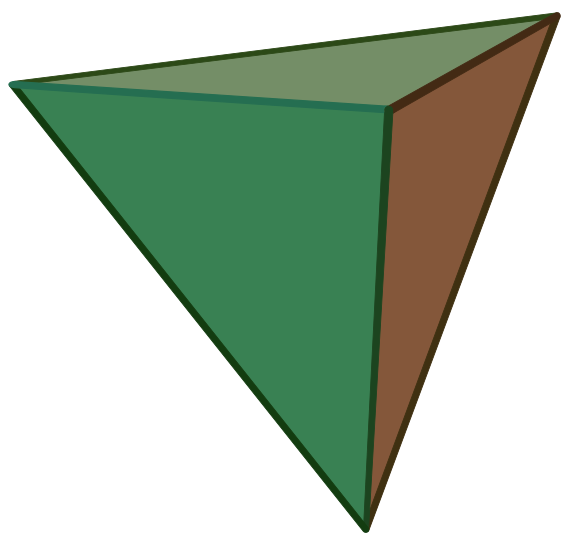
\includegraphics[width=0.25\marginparwidth]{SM/Tetrahedron.png}
\vspace*{-0.25cm}
\begin{center}\normalfont\small {Le Tétraèdre (le Feu).}\end{center}
\vspace*{-0.25cm}
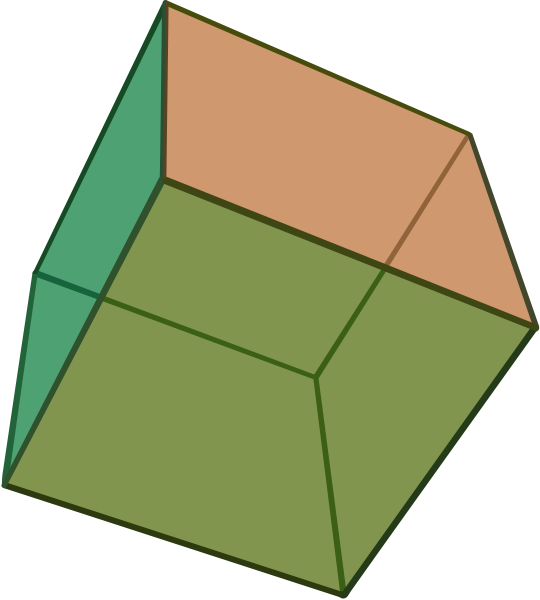
\includegraphics[width=0.25\marginparwidth]{SM/Hexahedron.png}
\vspace*{-0.25cm}
\begin{center}\normalfont\small {Le Cube (la Terre).}\end{center}
\vspace*{-0.25cm}
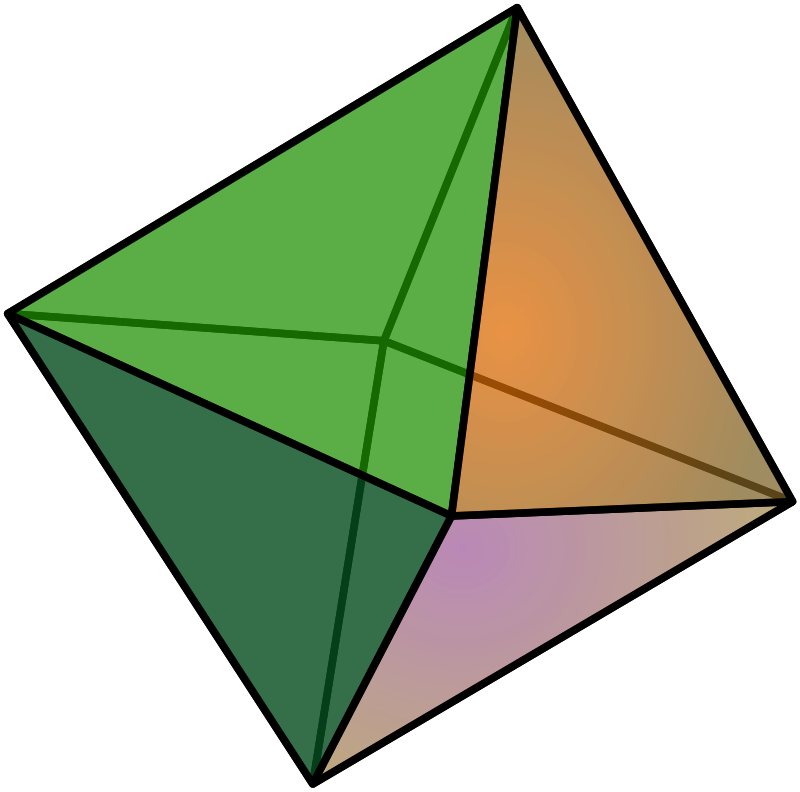
\includegraphics[width=0.25\marginparwidth]{SM/Octahedron.png}
\vspace*{-0.25cm}
\begin{center}\normalfont\small {L'Octaèdre (l'Air).}\end{center}
\vspace*{-0.25cm}
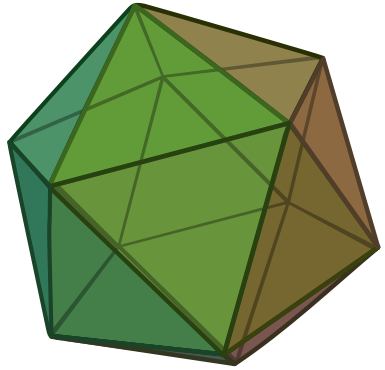
\includegraphics[width=0.25\marginparwidth]{SM/Icosahedron.png}
\vspace*{-0.25cm}
\begin{center}\normalfont\small {L'Icosaèdre (l'Eau).}\end{center}
\vspace*{-0.25cm}
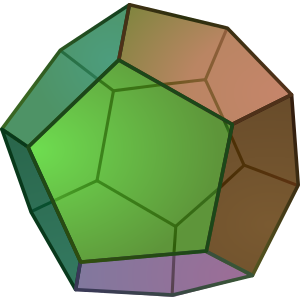
\includegraphics[width=0.25\marginparwidth]{SM/Dodecahedron.png}
\vspace*{-0.25cm}
\begin{center}\normalfont\small {Le Dodécaèdre (l'Univers).}\end{center}
\vspace*{-0.25cm}
\captionof{figure}{Les solides de Platon.}
\label{solides}
\end{center}
}
De tout temps les hommes ont voulu comprendre et maitriser la nature. Cette quête a amené de nombreux penseurs, et notamment les philosophes Grecs, à proposer des explications sur le monde qui nous entoure, et certaines de leurs idées se révéleront florisantes et donneront naissance des siècles plus tard à la Physique en tant que science au sens moderne du mot. 

Anaxagore (~500-428 av. J.C.) pronait que toute chose est formée de particules élémentaires. Cette idée sera reprise par Empédocle (~495-~435 av J.C) qui proposa, l'eau, la terre, l'air et le feu comme étant ces particules. Platon (428/427 - 348/347 av. J.C.) associera ces quatres éléménts aux polygones réguliers convexes de l'espace à trois dimension (le tétraèdre pour le Feu, le cube pour la Terre, l'octaèdre pour l'Air, l'icosaèdre pour l'Eau, le dodécaère reprèsente l'éther, élément constituant l'Univers (fig.\ref{solides})). On doit à Leucippe (~460-~370 av J.C.) et son disciple Démocrite (~460-~370 av J.C.) le concept d'atomes qui composent la matière et sont indivisibles et séparés par du vide. La véracité de l'atomisme fera débat pendant des siècles et ne sera validé expérimentalement qu'au cours du XIX\ieme siècle.

 Parmis les travaux les plus importants qui prouverons l'existence des atomes, citons ceux de Lavoisier (1743-1794) qui décompose de nombreuses substances en "Éléments". De nombreux travaux sur les gaz, la cristallographie, la physique statistique et la thermodynamique : Bernoulli (1700-1782) : cinétique des gaz, Haüy (1743-1822) : La forme des cristaux reflète la symétrie des "briques élémentaires" le constituant , Dalton (1766-1844) : symbolisation des corps simples et des corps composés par des symboles auxquels il donne un poids de matière (fig.\ref{atom}), et liste des masses atomiques d'un certain nombre d'éléments rapportés à la masse de l'hydrogène, Gay-Lussac (1778-1850) : les rapports des volumes des réactifs et des produits de réaction sont des nombres entiers petits , Maxwell(1831-1879) : dispersion statistique des vitesses des molécules, Boltzmann (1844-1906) : répartition statistique des vitesses dans un gaz , Mendeleïev : Classification périodique des éléments et prédiction de nouveaux atomes (fig.\ref{periodique}). Ces travaux feront passer petit à petit cette théorie en réalité scientifique. 
 
\marginpar
{
	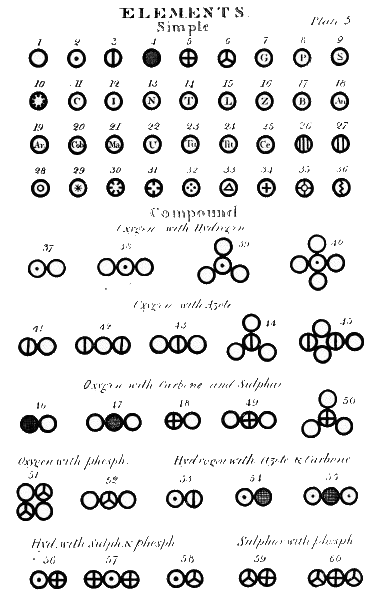
\includegraphics[width=\marginparwidth]{SM/Dalton.png}
    \captionof{figure}{Dessins de divers atomes et molécules tirés de l'ouvrage \textit{A New System of Chemical Philosophy}}
    	\label{atom}
}
\marginpar
{
	\vspace{2cm}
		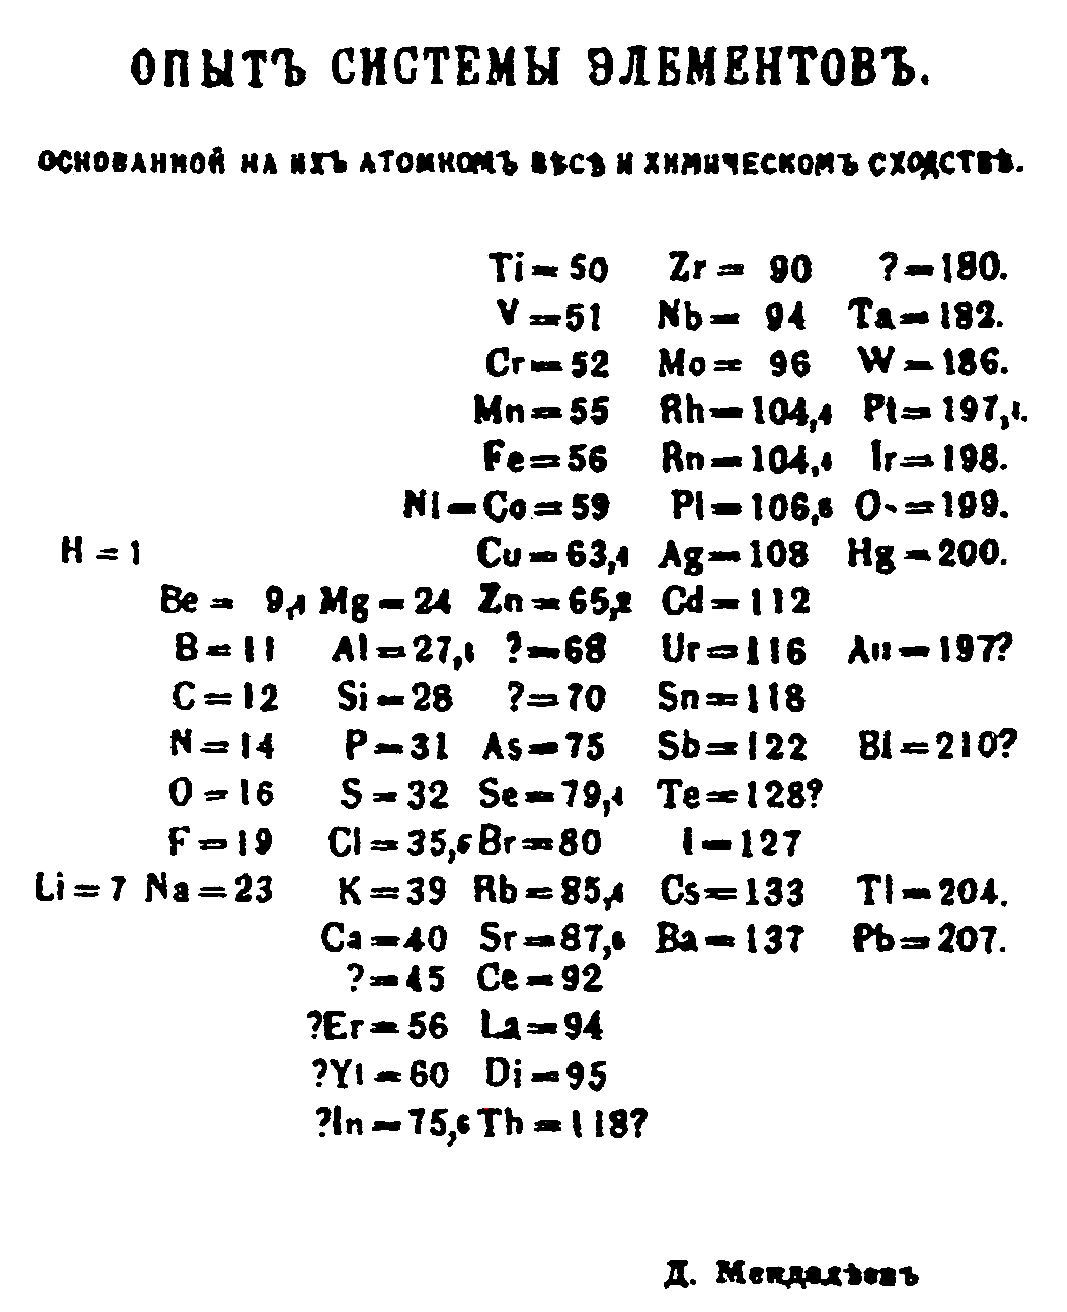
\includegraphics[width=\marginparwidth]{SM/periodique.png}
    \captionof{figure}{Tableau périodique de Mendeleïev}
    	\label{periodique}
}
D'autres domaine de la Physique connaitront des bouleversements importants au cours des siècles : 

Pour la Mécanique et la cosmologie : Copernic (1473-1543) et Galilée (1564-1642) : Modèle héliocentrique, Tycho Brahe (1546-1601) : remise en cause de  l'immuabilité du monde supra-lunaire énoncée par Aristote, Kepler (1571-1630) : Orbite elliptique des planètes, Newton (1643-1727) : théorie de la gravitation universelle, Lagrange (1736-1813) et Hamilton (1805-1865) : Principe de moindre action, Lagrangien, Hamiltonien.

Pour l'électromagnétisme : Coulomb(1736-1806) : loi de Coulomb, Volta(1745-1827): pile voltaïque, Ørsted (1777-1851), Ampère(1775-1836), Faraday(1792-1867), Henry (1797-1878) : les phénomènes d'induction, Maxwell : Équations de Maxwell.

Avec la découverte de l'électron par Thomson (1856-1940) en 1887 qui fût prédit en 1874 par Laming et Stoney. Thomson développe le premier modèle de l'atome, qui est décrit comme une boule de charge nulle possédant un noyau positif avec des électrons négatifs (modèle du "plum-pudding"). On découvre également durant cette période la radioactivité (Becquerel (1852-1908)). La physique semble à cette époque complète et cohérente. Lord Kelvin dira même dans son discours à la "Royal Institution of Great Britain" : \textit{"The beauty and clearness of the dynamical theory, which asserts heat and light to be modes of motion, is at present obscured by two clouds."}. Ces deux "nuages", l'incapacité à détecter l'éther luminifère  (expérience de Michelson-Morley) et la catastrophe ultraviolette du corps noir, donneront naissance respectivement à la relativité restreinte et à la mécanique quantique et feront entrer les physiciens dans la Physique Moderne.

Le début du siècle dernier sera une période florissante pour la physique des particules. Planck (1858-1947), afin de résoudre le problème du corps noir, proposera de quantifier les rayonnements : ceux-ci ne peuvent être qu'un multiple d'une constante qui porte son nom ($h$). Einstein ira plus loin et expliquera durant l'\textit{Annus mirabilis} (1905) l'effet photoélectrique en proposant le photon comme quanta de lumière qui agit comme une particule. Il possera également les bases de la relativité restreinte cette même année, réfutant le concept d'éther. De nombreux physiciens vont ensuite poser les bases de la mécanique quantique: Bohr (1885-1962), Compton (1892-1962), De Broglie (1892-1987), Schrödinger (1887-1961), Heisenberg (1901-1976), Dirac (1902-1984), Pauli (1900-1958). Avec les progrès tant théoriques qu'instrumentaux de Physiciens tels  Rutherford (1871-1937), Chadwick (1891-1974), Fermi (1901-1954), qui explorent le monde subatomique, on découvre les deux forces agissant à l'échelle du subatomique (les forces faible et forte) qui s'ajoutent aux deux force connues à l'époque (la force gravitationnelle et la force électromagnétique). Des physiciens tel Schwinger (1918-1994) veulent continuer la réunification des forces déjà avancée par les travaux de Maxwell ( force éléctrique et magnétique). Dans les années 1960, Weinberg (1933) et Salam (1926-1996) et Glashow (1932), réunissent dans une théorie dite électrofaible les forces électromagnétique et faible. Cette théorie prédit trois bosons ($W^{+}$, $W^{-}$ et $Z^{0}$). Leur théorie nécessite un boson supplémentaire, le boson de Higgs, postulé en 1964 par Brout, Englert, Higgs, Haggen Guralnik et Kibble afin de donner une masse aux particules. Cette théorie est la base du Modèle Standard de la physique des particules. La découverte des quarks amène à la création de la Chromodynamique Quantique (QCD) par Politzer (1949), Wilczek (1951), Gross (1941) afin de décrire l'interaction forte. Elle sera ensuite intégrée au Modèle Standard.

À partir de la seconde moitié du XX\ieme siècle, la Physique Subatomique a tâché de valider cette théorie et notamment par la découverte des bosons  $W^{+}$,$W^{-}$ et $Z^{0}$ en 1983, du quarks top $t$ en 1995, du neutrino tauique en 2000 et du boson de Higgs $h$ en 2012. De nombreux efforts sont également mené afin de continuer l'unification des forces entre elles. On sait cependant que le Modèle Standard, bien que jamais mis en défaut, ne peut tout expliquer. Certaines questions restent ouvertes et cette théorie présente même quelques défauts. La technicouleur, des modèles avec des dimensions supplémentaires ou la Supersymétrie sont des théories d'extension du Modèle Standard. Mais aucune n'a pu être encore validée expérimentalement.

\section{Le Modèle Standard de la physique des particules}
 
Au début du siècle dernier, tout tendait à faire croire que le monde était simplement composé d'atomes; eux mêmes constitués d'électron tournant autour d'un noyau composé de protons et neutrons. Tous les atomes connus avait été soigneusement classés dans le tableau périodique de Mendeleiev. Cependant, grâce à l'invention d'accélérateurs de particules linéaires, cyclotrons (fig. \ref{cyclo}) puis synchrotrons et l'observation des rayons cosmiques, les physiciens découvrirent bientôt qu'une pléthore de particules instables pouvaient être créées durant des désintégrations. Les Physiciens tentèrent bientôt de créer et classer ces particules en utilisant des énergies de faisceau de plus en plus grandes. Ce qui amena à la découverte d'une sous structure au sein même des nucléons\footnote{Protons et neutrons.} qui composent le noyau : les quarks (\ref{structure}).
\marginpar
{
	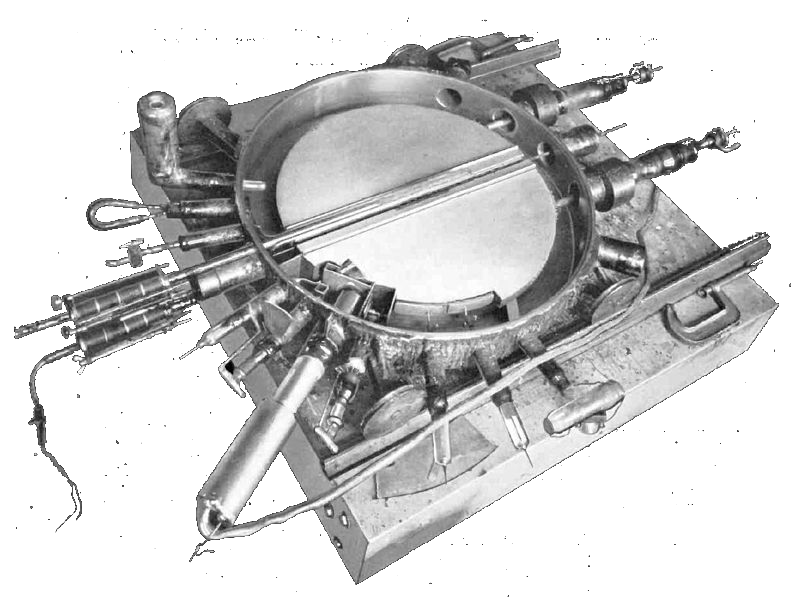
\includegraphics[width=\marginparwidth]{SM/cyclotron.png}
    \captionof{figure}{cyclotron de 27 pouces, accélérateur de $^{2}$H à 4 Mev (Université de Berkley, 1932).}
    	\label{cyclo}
}
\begin{figure}[h!]
\centering
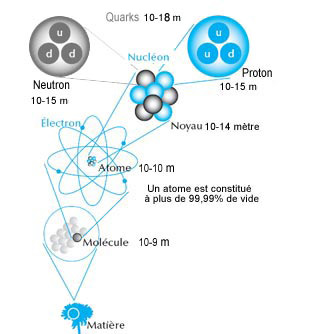
\includegraphics[width=0.55\textwidth]{SM/structure.jpg}
\captionof{figure}{Structure de la matière à différentes échelles.}
\label{structure}
\end{figure}

Parallèlement, de nouvelles interactions furent découvertes. Elles expliquaient les désintégrations radioactives ainsi que la cohésion des protons et des neutrons au sein du noyau atomique.

La physique des particules peut se résumer à la combinaison des deux démarches précédentes, à savoir, trouver les particules élémentaires ainsi que trouver les interactions fondamentales que ces particules peuvent subir. La manière dont ces particules interagissent aux moyens de ces interactions est donnée par la formulation mathématique d'une théorie, le Modèle Standard.

\subsection{Les particules élémentaires}
Les particules élémentaires du Modèle Standard, supposées indivisibles\footnote{à ce jour}, peuvent être classées en deux catégories selon leur spin (une propriété quantique intrinsèque à chaque particule) :
\begin{itemize}[label=$\bullet$]
\item les \textit{fermions}, ils constituent la matière et sont de spin demi-entier.
\item les \textit{bosons}, ils sont les messagers de l'interaction et sont de spin entier.
\end{itemize}
Chaque particule du Modèle Standard possède des nombres quantiques telles que sa masse, sa charge électrique, en fraction de l'opposé de la charge électrique de l'électron e par convention (e=$1.6\times10^{-19}$ C). Dans le cadre de la théorie, à chaque particule correspond une anti-particule\footnote{Une particule peut être sa propre anti-particule.} qui possède la même masse mais dont les nombres quantiques sont opposés.

\subsubsection{Les fermions}
Les fermions peuvent être classés en deux catégories selon qu'ils sont sensibles à l'interaction forte ou non. Dans le premier cas, ils font partis des \textit{quarks}, sinon ce sont des \textit{leptons}. Ces deux catégories sont elles-mêmes divisées en trois \textit{générations} (tab. \ref{fermions}).

Les leptons ont une charge électrique entière ($\pm$ 1) pour les électrons, muons et tau, et une charge nulle pour les neutrinos électroniques, neutrinos muoniques et neutrinos tauiques.

Les quarks ont une charge électrique fractionnaire. On associe à chaque quark un nombre quantique appelé "couleur" (Rouge, Vert et Bleu). Dû à la propriété de confinement de couleur, un quark ne peut être isolé et doit se combiner avec un ou deux autre quarks afin de former des \textit{mésons} (fig.\ref{mésons}) et des \textit{baryons} (fig.\ref{baryons}) respectivement. La somme des deux (trois) couleurs des quarks doit constituer un méson (baryon) "blanc" \footnote{Selon l'analogie avec la synthèse additive des couleurs.}. Les mésons et baryons sont regroupés sous le terme générique de \textit{hadrons}.
\marginpar
{
\centering
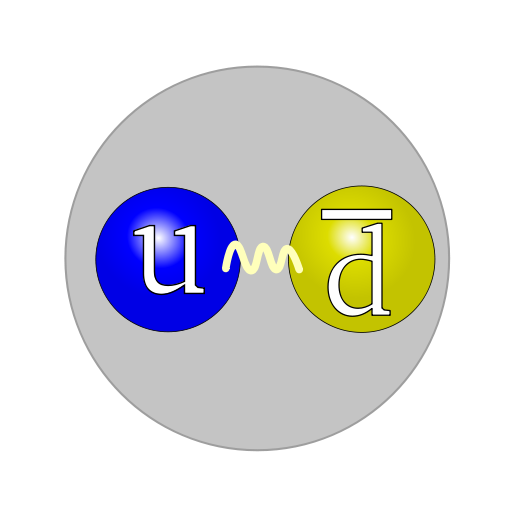
\includegraphics[width=\marginparwidth]{SM/quarks2.png}
\captionof{figure}{Un méson ($\pi^{+}$).}
\label{mésons}
}
\marginpar
{
    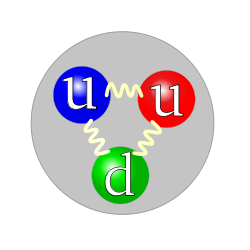
\includegraphics[width=\marginparwidth]{SM/quarks.png}
    \captionof{figure}{Un baryon ($p$).}
    	\label{baryons}
}	
\marginpar
{
\hspace*{-0.5cm}
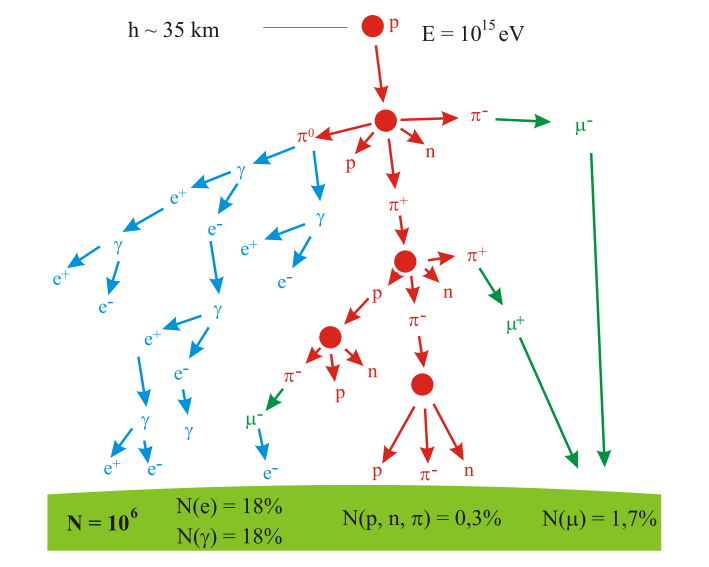
\includegraphics[width=1.2\marginparwidth]{SM/shower.png}
\captionof{figure}{Schéma d'une gerbe atmosphèrique.}
\label{gerbe}
}
La matière qui nous entoure n'est composée que de particules de la première génération. Tous les atomes sont composés d'électrons et de quarks $u$ et $d$ qui s'assemblent pour donner des protons $p$ et neutrons $n$. Les autres particules peuvent être créées si l'énergie disponible est suffisante (lors de gerbe atmosphérique où un proton vient interagir avec des particules de notre atmosphère par exemple \ref{gerbe} ou dans un collisionneur).
\definecolor{Orange}{HTML}{FFDD00}
\definecolor{Orange2}{HTML}{FFC000}
\definecolor{Green}{HTML}{8FB73E}
\definecolor{Green2}{HTML}{4EA700}
\definecolor{Red}{HTML}{EF4123}
\definecolor{Red2}{HTML}{EF2300}
\newcolumntype{P}[1]{>{\centering\arraybackslash}p{#1}}
\begin{table}[H]
\centering
\begin{tabular}{|S{P{15mm}}|S{P{39mm}}|S{P{39mm}}|S{P{39mm}}|}
\hline 
\rowcolor{Orange2}Quarks & 1\iere génération & 2\ieme génération & 3\ieme génération \\
\hline 
\cellcolor{Orange2}\shortstack{ Nom \\ Notation \\ Charge \\ Masse}& \cellcolor{Orange}\shortstack{ Up \\ $u$,$\bar{u}$ \\ $\pm \frac{2}{3}$ \\ $0.005$ GeV/c$^2$} & \cellcolor{Orange}\shortstack{ Charm \\ $c$,$\bar{c}$ \\ $\pm \frac{2}{3}$ \\ $1.35$ GeV/c$^2$}&\cellcolor{Orange}\shortstack{ Top \\ $t$,$\bar{t}$ \\ $\pm \frac{2}{3}$ \\ $172.6$ GeV/c$^2$}\\
\hline 
\cellcolor{Orange2}\shortstack{ Nom \\ Notation \\ Charge \\ Masse}& \cellcolor{Orange}\shortstack{ Down \\ $d$,$\bar{d}$ \\ $\mp \frac{1}{3}$ \\ $0.01$ GeV/c$^2$}& \cellcolor{Orange}\shortstack{ Strange \\ $s$,$\bar{s}$ \\ $\mp \frac{1}{3}$ \\ $0.1$ GeV/c$^2$}& \cellcolor{Orange}\shortstack{ Bottom \\ $b$,$\bar{b}$ \\ $\mp \frac{1}{3}$ \\ $1.3$ GeV/c$^2$}\\
\hline 
\rowcolor{Green2} Leptons & 1\iere génération & 2\ieme génération & 3\ieme génération \\
\hline
\cellcolor{Green2}\shortstack{ Nom \\ Notation \\ Charge \\ Masse}& \cellcolor{Green}\shortstack{ Électron \\ $e^{\pm}$ \\ $\pm 1$ \\ $0.511$ MeV/c$^2$}& \cellcolor{Green}\shortstack{ Muon \\ $\mu^{\pm}$ \\ $\pm 1$ \\ $105.7$ MeV/c$^2$}& \cellcolor{Green}\shortstack{ Tau \\ $\tau^{\pm}$ \\ $\pm 1$ \\ $1777$ MeV/c$^2$}\\
\hline 
\cellcolor{Green2}\shortstack{ Nom \\ Notation \\ Charge \\ Masse }& \cellcolor{Green}\shortstack{ Neutrino électronique \\ $\nu_{e}$ \\ $0$ \\ $<0.017$ MeV/c$^2$}& \cellcolor{Green}\shortstack{ Neutrino muonique \\ $\nu_{\mu}$ \\ $0$ \\ $<0.27$ MeV/c$^2$}&\cellcolor{Green}\shortstack{ Neutrino tauique \\ $\nu_{\tau}$ \\ $0$ \\ $<35$ MeV/c$^2$}\\
\hline
\end{tabular} 
\captionof{table}{Fermions: Quarks et Leptons.}
\label{fermions}
\end{table}	

\subsubsection{Les bosons}
La description perturbative du Modèle Standard utilise l'échange de bosons virtuelles, afin de décrire l'interaction entre deux particules. Les bosons sont les médiateurs des interactions. Les particules de matière (fermions) interagissent donc entre elles par l'échange de particules de spin 1 correspondant à la force responsable de leur interaction.
\smallskip
Chacune des quatre interactions possède donc un ou plusieurs bosons appelés bosons de jauge (bosons vecteurs) (Tab.\ref{bosons}) :
\marginpar
{
\begin{center}
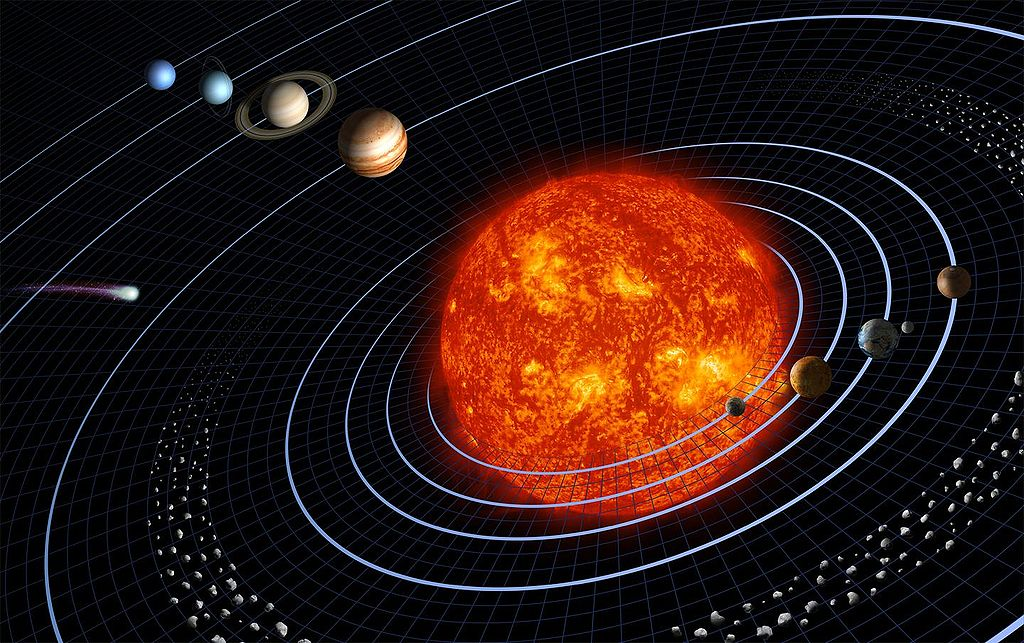
\includegraphics[width=\marginparwidth]{SM/solaire.jpg}
\begin{center}\normalfont\small {(a) Gravité : Système solaire.}\end{center}
\end{center}
}
\marginpar
{
\begin{center}
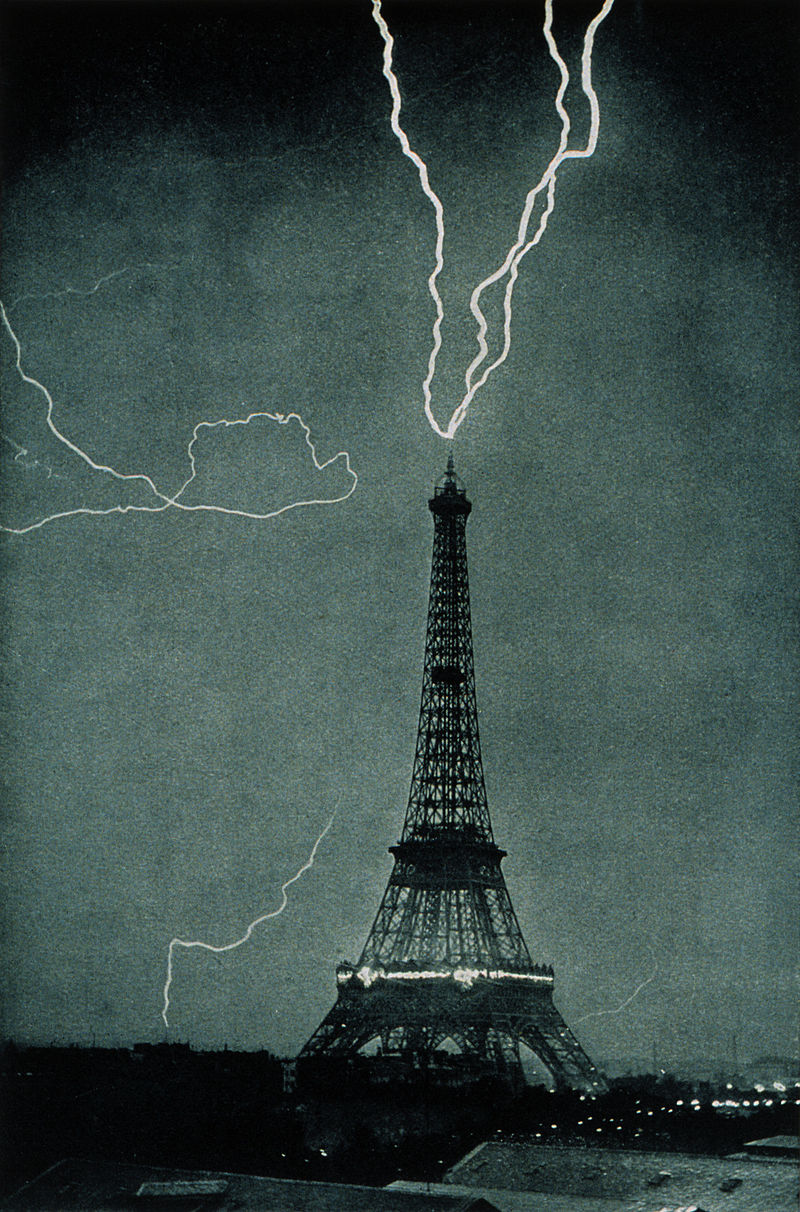
\includegraphics[width=\marginparwidth]{SM/foudre.jpg}
\begin{center}\normalfont\small {(b) Électromagnétisme : la foudre.}\end{center}
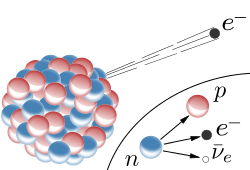
\includegraphics[width=\marginparwidth]{SM/beta.png}
\begin{center}\normalfont\small {(c) Interaction faible : désintégration $\beta$.}\end{center}
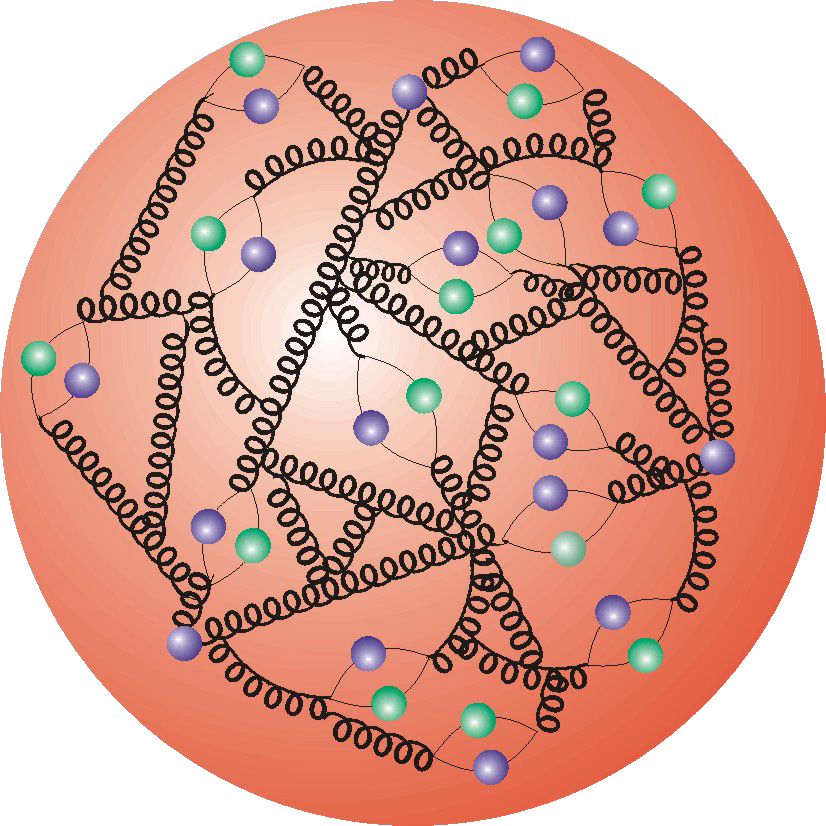
\includegraphics[width=0.8\marginparwidth]{SM/quarks3.png}
\begin{center}\normalfont\small {(d) Interaction forte : confinement.}\end{center}
\captionof{figure}{Exemple d'effets des 4 interactions.}
%\label{solides}
\end{center}
}
\begin{itemize}[label=$\bullet$]
\item \textbf{L'interaction gravitationnelle} est la première à avoir été découverte et expliquée (Galilée, Newton). Elle est négligeable à l'échelle atomique. Elle est gouvernée par la masse des corps mise en jeu et elle domine à grande échelle ( Univers, Galaxies, Planètes), son rayon d'action est infini. Sa description quantique repose sur un boson de spin 2 qui est encore activement recherché. Un pas décisif à été fait grâce à la détection par les expériences Virgo et Ligo des ondes Gravitationnelle. Cette interaction est la seule à ne pas être intégrée au Modèle Standard. Elle est actuellement décrite par la Relativité Générale qui est une approche non quantique.

\item \textbf{L'interaction électromagnétique} gouverne les interactions entre les particules chargées. C'est l'une des interactions qui nous est la plus familière car elle est prépondérante dans notre vie quotidienne ( lumière, chimie, frottements ...). Tout comme la gravité, son rayon d'action est infini. Son boson médiateur est le photon $\gamma$.

\item \textbf{L'interaction faible} à été découverte et comprise à travers la désintégration de particules avec changements de saveurs. Elle fait passer d'un fermion à un autre (par exemple lors de la désintégration $\beta$, elle transforme un neutron en un proton en changeant un quark $d$ en un quark $u$ avec la création d'un neutrino et d'un électron). Les bosons médiateurs de l'interaction sont les bosons $W^{+}$ $W^{-}$ $Z^{0}$. Sa portée est de l'ordre de 10$^{-18}$ m due à la masse des bosons médiateur.

\item \textbf{L'interaction forte} permet l'échange de couleur entre les quarks et la création et l'annihilation de particules. Elle est responsable de la cohésion du noyau, et elle lie les nucléons entre eux à l'intérieur du noyau atomique. Ses bosons médiateur sont les gluons et sont au nombre de huit. Bien que les gluons soient supposés de masse nulle, la portée de l'interaction est de l'ordre de 10$^{-15}$ m. Cette portée est la conséquence du principe de confinement de couleur qui affecte les quarks. En effet, cette interaction a la propriété de voir son intensité augmenter avec la distance, ce qui à tendance à regrouper les quarks entre eux. Cette propriété est également responsable du processus d'hadronisation des quarks et de la création de jets.
\end{itemize}
\smallskip
\begin{table}[h!]
\centering
\begin{tabular}{|S{P{33mm}}|S{P{26mm}}|S{P{22mm}}|S{P{52mm}}|}
\hline 
\rowcolor{Red2}Interaction&Rayon d'action&Bosons de jauge&Masses\\
\hline 
\cellcolor{Red}\shortstack{ Forte }&
\cellcolor{Red}\shortstack{ $2.5\times10^{-15}$ m}& 
\cellcolor{Red}\shortstack{  Gluons (8)}&
\cellcolor{Red}\shortstack{ 0}\\
\hline 
\cellcolor{Red}\shortstack{ Electromagnétique }&
\cellcolor{Red}\shortstack{ $\infty$}& 
\cellcolor{Red}\shortstack{Photon $\gamma$}&
\cellcolor{Red}\shortstack{0}\\
\hline 
\cellcolor{Red}\shortstack{Faible}&
\cellcolor{Red}\shortstack{$10^{-18}$ m }& 
\cellcolor{Red}\shortstack{$W^{\pm}$,$Z^{0}$}&
\cellcolor{Red}\shortstack{$80.399$ Gev/c$^{2}$,$91.188$ Gev/c$^{2}$ }\\
\hline 
\cellcolor{Red}\shortstack{Gravitationnelle}&
\cellcolor{Red}\shortstack{$\infty$}& 
\cellcolor{Red}\shortstack{(Graviton)}&
\cellcolor{Red}\shortstack{(inconnue)}\\
\hline 
\end{tabular} 
\captionof{table}{Bosons : Interactions.}
\label{bosons}
\end{table}

\subsubsection{Le boson de Higgs}
Le boson de Higgs ($H^{0}$) est nécessaire afin de donner la masse des bosons $W^{\pm}$, $Z^{0}$ et des fermions. Bien que postulé en 1964, il n'a été découvert qu'en 2012 par les expériences CMS et ATLAS en 2012. Contrairement au bosons vecteur, le boson de Higgs est de spin 0.
\newpage
Toutes ces particules peuvent être résumer dans le tableau suivant : 

\begin{minipagewithmarginpars}[h]{\textwidth}
\vspace{-0.5cm}
\centering
\hspace*{-1.5cm}
\includestandalone{./SM/bestiaire}
\captionof{figure}{Classification des quarks, leptons et bosons.}
\label{bestiaire}
\marginpar
{
\vspace*{1.5cm}
\begin{center}
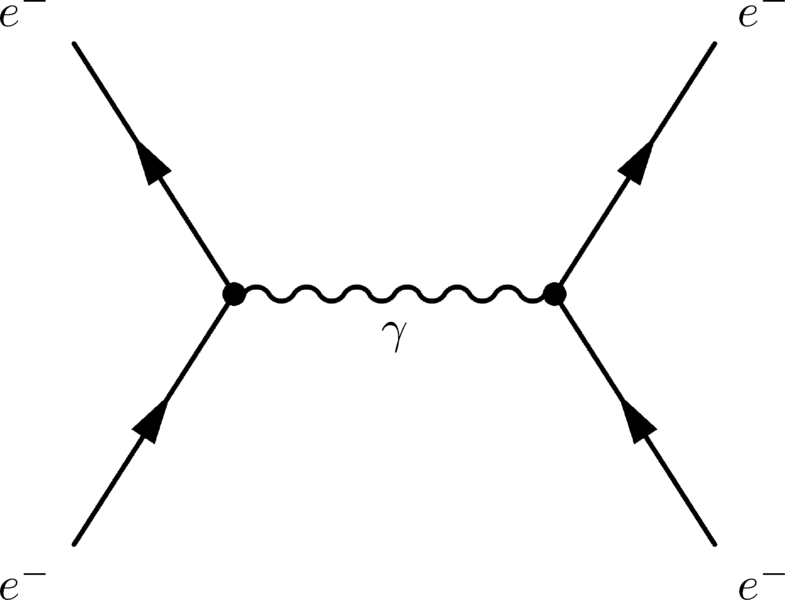
\includegraphics[width=\marginparwidth]{SM/feyn0.png}
\begin{center}\normalfont\small {(a) Développement à l'arbre.}\end{center}
\end{center}
}
\end{minipagewithmarginpars}
\subsection{Le formalisme du Modèle Standard}
\marginpar
{
\centering
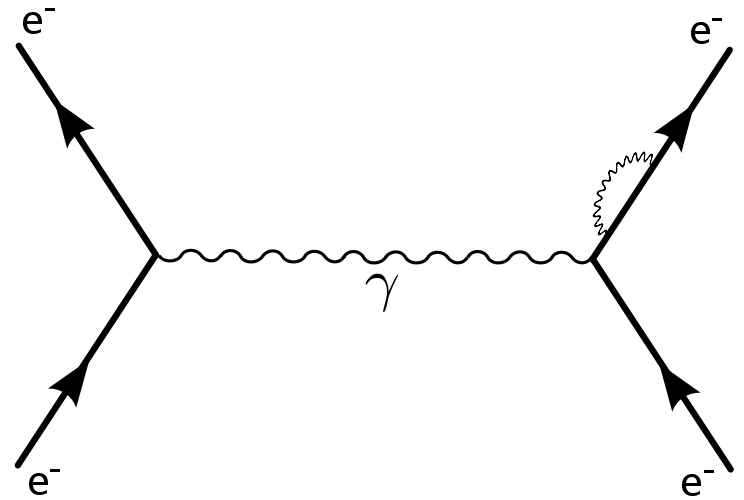
\includegraphics[width=\marginparwidth]{SM/feyn1.png}
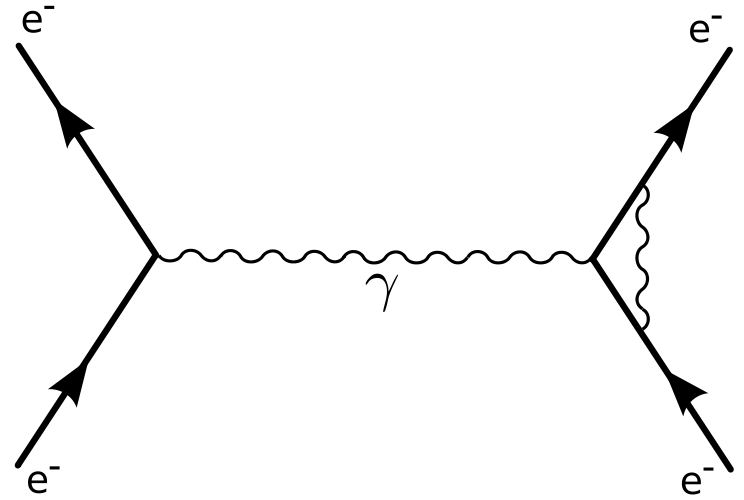
\includegraphics[width=\marginparwidth]{SM/feyn2.png}
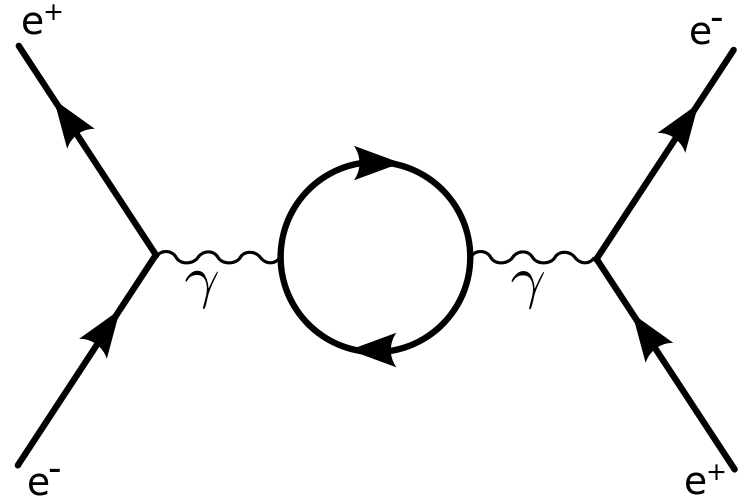
\includegraphics[width=\marginparwidth]{SM/feyn3.png}
\begin{center}\normalfont\small {(b) Développement à l'ordre 1.}\end{center}
\captionof{figure}{Exemple de diagrammes de Feynman pour le développement en série de la diffusion électron-électron.}
\label{feyn}
}
Le Modèle Standard est une théorie non-abélienne où les interactions sont régis par des symétries locales de jauge. Elle repose sur la théorie quantique des champs qui permet de décrire les particules et leurs interactions. Cette théorie est à la fois quantique et relativiste. Elle permet donc de caractériser les interactions par des probabilités de transition d'un état initial à un état final, ainsi que de rendre compte du temps de propagation des interactions, la description des particules à hautes énergie et les créations annihilation de particules.

Dans cette théorie, à chaque type de particule est associé un champ $\psi(\vec{x},t)$ et les interactions sont liées à des propagateurs. La création (l'annihilation) de particules est associé à des opérateurs qui excitent(désexciter) le champ de particules à une position $\vec{x}$ et à un temps $t$. L'un des postulat de la théorie quantique des champs est que l'ensemble des informations de la théorie est contenu dans un Lagrangien $\mathcal{L}$ qui s'exprime en fonction des champs et de leurs dérivées. Il est possible, à partir de ce Lagrangien d'obtenir les équations de mouvements en minimisant sont action $S=\int\mathcal{L}\Diff4{x}$.
Le Modèle Standard et une théorie perturbative, c'est à dire que les observables sont calculées par une méthode qui s'appuie sur un développement en série dont la précision augmente avec l'ordre. Au premier ordre, l'observable est dite être calculé à l'arbre ou LO (Leading Order). Ce développement en série n'est valable que si les constantes de couplage des interactions reste faible devant l'unité. Ce développement en série peut être schématisé grâce aux diagrammes de Feynmann (fig. \ref{feyn}), qui sont des diagramme représentant des règles de calculs. Chaque types de particules et d'interactions posséde son symbole et à chaque particules doit être connécté par un vertex (représentant une interactions).

Le principe selon lequel les interactions sont gouvernés par des symétries est également un postulat des important du Modèle Standard. De par le théorème de Noether, les symétries continues sont liées à des quantités physique qui se conserve. Le Modèle Standard est basé sur le produit direct du groupe de la chromodynamique quantique, décrivant l'interaction forte, qui impose une conservation de la charge de couleur, $SU(3)_{C}$ et du groupe de la théorie électrofaible, $SU(2)_{L} \otimes U(1)_{Y}$, imposant une symétrie locale de l'isospin $I$ associé au groupe $SU(2)_{L}$ et une symètrie locale de l'hypercharge $Y$ du groupe $U(1)_{Y}$.

\subsection{Lagrangien du modèle standard}
Le modèle standard est une théorie de Jauge qui se base sur le groupe $SU(3)_{C} \otimes SU(2)_{L} \otimes U(1)_{Y}$ dont le lagrangien peut s'écrire sous la forme :

\begin{equation}
\mathcal{L_{MS}}=\mathcal{L}_{\mathrm{Yang-Mills}}+\mathcal{L}_{\mathrm{Dirac}}+\mathcal{L}_{\mathrm{Yukawa}}+\mathcal{L}_{\mathrm{Higgs}}
\end{equation}

\subsubsection{Le terme de Yang-Mills (secteur de jauge)}
Le secteur de jauge est la partie cinématique des champs de jauge :
\begin{equation}
\mathcal{L}_{\mathrm{Yang-Mills}}=-\frac{1}{4}B_{\mu\nu}B^{\mu\nu}-\frac{1}{4}W_{\mu\nu}^{a}W_{a}^{\mu\nu}-\frac{1}{4}G_{\mu\nu}^{A}G_{A}^{\mu\nu}
\end{equation}
où 
\begin{equation}
B_{\mu\nu}=\partial_{\mu}B_{\nu}-\partial_{\nu}B_{\mu}
\end{equation}
avec $B_{\mu}$ le champ isoscalaire associé au groupe d'hypercharge $U(1)_{Y}$,
\begin{equation}
W_{\mu\nu}^{a}=\partial_{\mu}W_{\nu}^{a}-\partial_{\nu}W_{\mu}^{a}+g\epsilon_{abc}W_{\mu}^{b}W_{\nu}^{c}
\end{equation}
où $W_{\mu}^{a} (a=1,2,3)$ est le triplet d'isospin I=1 du groupe de l'isospin faible $SU(2)_{L}$, g la constante de couplage de l'isospin faible et $\epsilon_{abc}$ les constantes de structures antisymétriques correspondantes.  
\begin{equation}
G_{\mu\nu}^{A}=\partial_{\mu}G_{\nu}^{A}-\partial_{\nu}G_{\mu}^{A}+g'\epsilon_{ABC}G_{\mu}^{B}G_{\nu}^{C}
\end{equation}
les champs des gluons $G_{\mu}^{A} (A=1,2,..,8)$, bosons vecteurs de $SU(3)_{c}$, $g'$ la constante de couplage de couleur et $f_{ABC}$ les constantes de structures de $SU(3)_{C}$.
La nature non-Abélienne de $SU(2)_{L}$ et $SU(3)_{c}$ amène à des termes supplémentaires dans l'écriture des champs du triplet d'isospin et des champs de gluons. Ce sont ces termes qui sont reponsables de l'interaction des bosons $W$ et des gluons $g$.

\subsubsection{Le secteur de Dirac}
Le secteur de Dirac décrit les interactions des fermions avec les bosons de jauge. Dans le secteur électrofaible, les fermions se regroupent de manière asymétrique dans des doublets d'isospin faible de chiralité gauche et dans des singulets de chiralité droite (tab. \ref{doublets}). Il y a violation maximale de la parité de $SU(2)_{L}\otimes U(1)_{Y}$

\begin{table}[H]
\centering
\begin{tabular}{|Sc|Sc|} 
\hline
\multicolumn{2}{|Sc|}{Quarks} \\
\hline
Gauches $Q_{\alpha L}^{i}$ & $\begin{pmatrix} 
u^{i}\\
d^{i}
\end{pmatrix}_{L},\ \begin{pmatrix} 
c^{i}\\
s^{i}
\end{pmatrix}_{L},\ \begin{pmatrix} 
t^{i}\\
b^{i}
\end{pmatrix}_{L}$ \\
\hline
Droits $Q_{\beta R}^{i}$&$ u_{iR},\ d_{iR},\ c_{iR},\ s_{iR},\ t_{iR},\ b_{iR}$\\
\hline
\multicolumn{2}{|Sc|}{Leptons} \\
\hline
Gauche $L_{\alpha L}$& $\begin{pmatrix} 
\nu_{e}\\
e
\end{pmatrix}_{L},\ \begin{pmatrix} 
\nu_{\mu}\\
\mu
\end{pmatrix}_{L},\ \begin{pmatrix} 
\nu_{\tau}\\
\tau
\end{pmatrix}_{L} $\\
\hline
Droits $L_{\gamma R}$& $e_{R},\ \mu_{R},\ \tau_{R},\ \left(\nu_{e R},\ \nu_{\mu R},\ \nu_{\tau R}\right)$ \\
\hline
\end{tabular}
\captionof{table}{Doublets et singulets pour $SU(2)_{L}$ ;$i$=1,2,3 couleurs, $\alpha$=1,2,3 familles, $\beta$={u,d,s,c,t,b}, $\gamma$={$e$,$\mu$,$\tau$,$\left(\nu_{e},\nu_{\mu},\nu_{\tau}\right)$}}.
\label{doublets}
\end{table}	

En suivant ces notations le secteur de Dirac du Lagrangien du Modèle Standard s'écrit:
\marginpar
{
\begin{equation*}
\sigma_{1}=\begin{pmatrix} 
0&1\\
1&0\\
\end{pmatrix}
\end{equation*}
\vspace{0.2cm}
\begin{equation*}
\sigma_{2}=\begin{pmatrix} 
0&-i\\
i&0\\
\end{pmatrix}
\end{equation*}
\vspace{0.2cm}
\begin{equation*}
\sigma_{3}=\begin{pmatrix} 
1&0\\
0&-1\\
\end{pmatrix}
\end{equation*}
\captionof{figure}{Les matrices canoniques de Pauli.}
\label{Pauli}
}
\marginpar
{
\begin{equation*}
\lambda_{1}=\begin{pmatrix} 
0&1&0\\
1&0&0\\
0&0&0
\end{pmatrix}
\end{equation*}
\vspace{0.2cm}
\begin{equation*}
\lambda_{2}=\begin{pmatrix} 
0&-i&0\\
i&0&0\\
0&0&0
\end{pmatrix}
\end{equation*}
\vspace{0.2cm}
\begin{equation*}
\lambda_{3}=\begin{pmatrix} 
1&0&0\\
0&-1&0\\
0&0&0
\end{pmatrix}
\end{equation*}
\vspace{0.2cm}
\begin{equation*}
\lambda_{4}=\begin{pmatrix} 
0&0&1\\
0&0&0\\
1&0&0
\end{pmatrix}
\end{equation*}
\vspace{0.2cm}
\begin{equation*}
\lambda_{5}=\begin{pmatrix} 
0&0&-i\\
0&0&0\\
i&0&0
\end{pmatrix}
\end{equation*}
\vspace{0.2cm}
\begin{equation*}
\lambda_{6}=\begin{pmatrix} 
0&0&0\\
0&0&1\\
0&1&0
\end{pmatrix}
\end{equation*}
\vspace{0.2cm}
\begin{equation*}
\lambda_{7}=\begin{pmatrix} 
0&0&0\\
0&0&-i\\
0&i&0
\end{pmatrix}
\end{equation*}
\vspace{0.2cm}
\begin{equation*}
\lambda_{8}=\frac{1}{\sqrt{3}}\begin{pmatrix} 
1&0&0\\
0&1&0\\
0&0&-2
\end{pmatrix}
\end{equation*}
\captionof{figure}{Les matrices canoniques de Gell-Mann.}
\label{Gell-Mann}
}

\begin{equation}
\begin{split}
\mathcal{L}_{\mathrm{Dirac}}=&i\sum_{\alpha=1}^{3}\bar{L}_{\alpha L}\gamma_{\mu}D_{L_{L}}^{\mu}L_{\alpha L}+\sum_{\gamma=1}^{3(6)}\bar{L}_{\gamma R}\gamma_{\mu}D_{L_{R}}^{\mu}L_{\gamma R}\\
&+\sum_{\alpha=1}^{3}\sum_{i=1}^{3}\bar{Q}_{\alpha L}^{i}\gamma_{\mu}D_{Q_{L}}^{\mu}Q_{\alpha L}^{i}+\sum_{\beta=1}^{6}\sum_{i=1}^{3}\bar{Q}_{\beta R}^{i}\gamma_{\mu}D_{Q_{R}}^{\mu}Q_{\beta R}^{i}
\end{split}
\end{equation}
Avec les dérivées covariantes de la forme : 
\begin{equation}
D_{\mu L_{L}}=\partial_{\mu} -ig\frac{\sigma^a}{2}W_{\mu}^{a}-ig'\frac{Y^{W}_{L}}{2}B_{\mu}
\end{equation}
\begin{equation}
D_{\mu L_{R}}=\partial_{\mu} -ig'\frac{Y^{W}_{R}}{2}B_{\mu}
\end{equation}
\begin{equation}
D_{\mu Q_{L}}=\partial_{\mu} -ig\frac{\sigma^a}{2}W_{\mu}^{a}-ig'\frac{Y^{W}_{L}}{2}B_{\mu}-ig''\frac{\lambda^{A}}{2}Q_{\mu}^{A}
\end{equation}
\begin{equation}
D_{\mu Q_{R}}=\partial_{\mu}ig'\frac{Y^{W}_{R}}{2}B_{\mu}-ig''\frac{\lambda^{A}}{2}Q_{\mu}^{A}
\end{equation}
où $\sigma^{a}$ sont les générateur de $SU(2)_{L}$ (matrices de Pauli (Fig. \ref{Pauli})), $\lambda^{A}$ les générateurs de $SU(3)_{c}$ (matrices de Gell-Mann (Fig. \ref{Gell-Mann})) et $Y^{W}$, l'hypercharge faible, le générateur de $U(1)_{Y}$. 
Afin d'obtenir les charges électriques pour chaque fermions, on pose:
\begin{multline}
\begin{split}
&Y^W(L_{\alpha L})=-1,\ &Y^W(e_{R},\mu_{R},\tau_{R})=-2,\ &\left(Y^W(\nu_{e R},\nu_{\mu R},\nu_{\tau R})=0\right)\\
&Y^W(Q_{\alpha L})=\frac{1}{3},\ &Y^W(u_{R},c_{R},t_{R})=\frac{4}{3},\ &Y^W(d_{R},s_{R},b_{R})=-\frac{2}{3}
\end{split}
\end{multline}  

\subsubsection{Le secteur de Higgs} 
La symétrie électrofaible est incompatible avec la description de fermion massif. En effet, dans le Lagrangien les termes de masses des fermions sont de la forme 
\begin{equation}
\mathcal{L_{M}}=-m\bar{\phi}\phi=-m \left(\phi_{L}^{\dagger}\phi_{R}+\phi_{R}^{\dagger}\phi_{L}\right)
\end{equation}
Cependant, ces termes brisent la symétrie $SU(2)$ et n'est donc pas inclus dans le Lagrangien. De plus, l'expérience montre que les bosons de jauge $W$ doivent posséder une masse. Or l'introduction des termes de masses pour ces boson est également impossibles pour les mêmes raisons.

Afin de résoudre ces problèmes, on introduit un champ scalaire complexe $\phi$, doublet de $SU(2)_{L}$ de quatre champs réels $\phi_{i}$ et d'hypercharge $Y=1$ :
\begin{equation}
\phi=\begin{pmatrix} 
\phi^{+}\\
\phi^{0}
\end{pmatrix}=\frac{1}{\sqrt{2}}\begin{pmatrix} 
\phi_{1}+\phi_{2}\\
\phi_{3}+\phi_{4}
\end{pmatrix}
\end{equation}
On utilise l'expression du Lagrangien la plus générale pour un champ scalaire complexe de $SU(2)$:
\begin{equation}
\mathcal{L}_{\mathrm{Higgs}}=\left(D_{\mu}\phi\right)^{\dagger}\left(D^{\mu}\phi\right)-V(\phi),
\end{equation}
avec 
\begin{equation}
D_{\mu}=\partial_{\mu} -ig\frac{\sigma^a}{2}W_{\mu}^{a}-ig'\frac{Y}{2}B_{\mu}.
\end{equation}
Afin que le lagrangien $\mathcal{L}_{\mathrm{Higgs}}$ soit invariant globalement, le potentiel scalaire $V(\phi)$ ne doit pas comporter de puissance impaires de $\phi$. De plus, afin que la théorie reste renormalisable, les puissances au delà de $\phi^4$ sont à proscrire.

Le potentiel $V(\phi)$ est donc de la forme :
\begin{equation}
V(\phi)=\mu^{2}\phi^{\dagger}\phi+\lambda\left(\phi^{\dagger}\phi\right)^2,
\end{equation}
et a un profil différent selon les signes de $\mu^{2}$ et de $\lambda$ (Fig. \ref{profile}).
\marginpar{ 
\resizebox {\marginparwidth} {!} 
{
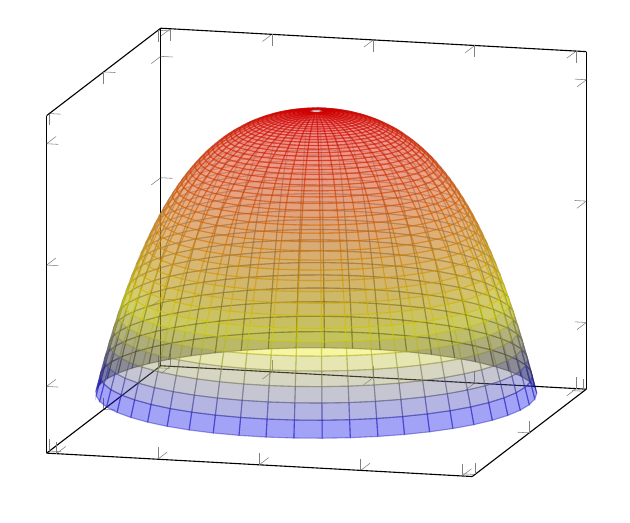
\begin{tikzpicture}
\begin{axis}[view={15}{15},yticklabels={,,},xticklabels={,,},zticklabels={,,},mesh/interior colormap name=hot,colormap/blackwhite]
\addplot3[surf,shader=faceted,samples=50,fill opacity=0.5,opacity=0.4,domain=0:1.05,y domain=0:2*pi,z buffer=sort]({x * cos(deg(y))}, {x * sin(deg(y))}, {-x*x-x*x*x*x});
\end{axis}
\end{tikzpicture}
}
\begin{center}\normalfont\small {(a) $\mu^{2}<0$ , $\lambda<0$.}\end{center}
\resizebox {\marginparwidth} {!} 
{
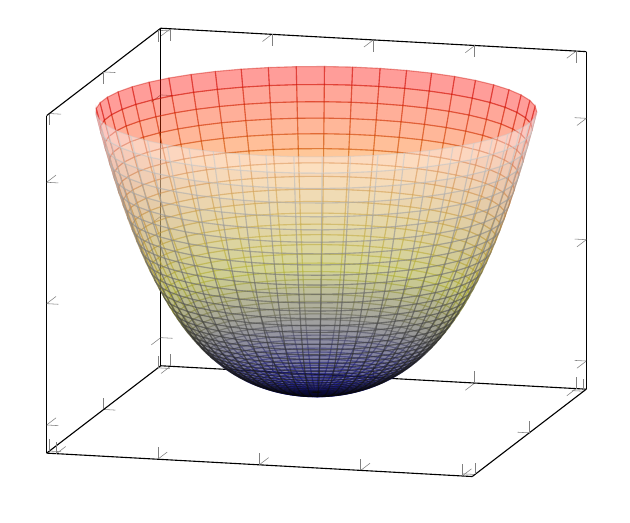
\begin{tikzpicture}
\begin{axis}[view={15}{15},yticklabels={,,},xticklabels={,,},zticklabels={,,},mesh/interior colormap name=hot,colormap/blackwhite]
\addplot3[surf,shader=faceted,samples=50,fill opacity=0.5,opacity=0.4,domain=0:1.05,y domain=0:2*pi,z buffer=sort]({x * cos(deg(y))}, {x * sin(deg(y))}, {+x*x+x*x*x*x});
\end{axis}
\end{tikzpicture}
}
\begin{center}\normalfont\small {(b) $\mu^{2}>0$ , $\lambda>0$.}\end{center}
\resizebox {\marginparwidth} {!} 
{
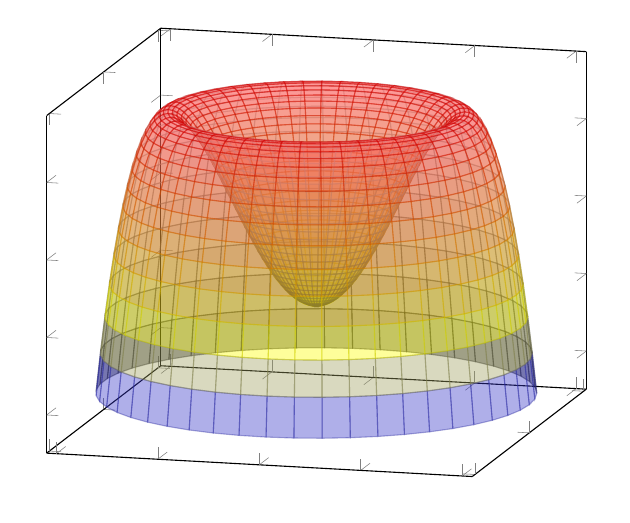
\begin{tikzpicture}
\begin{axis}[view={15}{15},yticklabels={,,},xticklabels={,,},zticklabels={,,},mesh/interior colormap name=hot,colormap/blackwhite]
\addplot3[surf,shader=faceted,samples=50,fill opacity=0.5,opacity=0.4,domain=0:1.05,y domain=0:2*pi,z buffer=sort]({x * cos(deg(y))}, {x * sin(deg(y))}, {+x*x-x*x*x*x});
\end{axis}
\end{tikzpicture}
}
\begin{center}\normalfont\small {(c) $\mu^{2}>0$ , $\lambda<0$.}\end{center}
\resizebox {\marginparwidth} {!} 
{
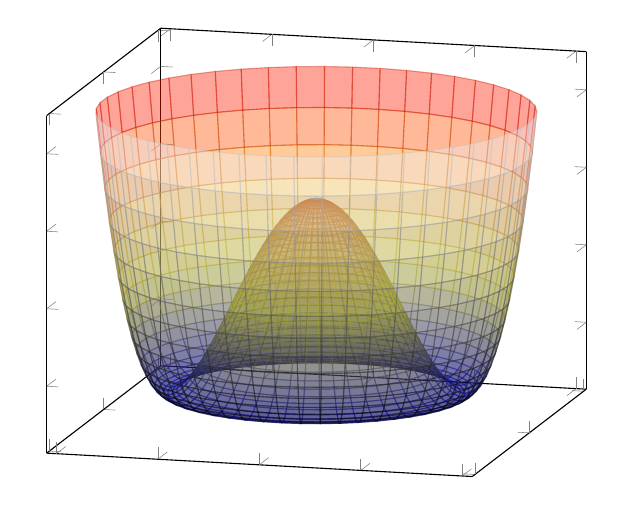
\begin{tikzpicture}
\begin{axis}[view={15}{15},yticklabels={,,},xticklabels={,,},zticklabels={,,},mesh/interior colormap name=hot,colormap/blackwhite]
\addplot3[surf,shader=faceted,samples=50,fill opacity=0.5,opacity=0.4,domain=0:1.05,y domain=0:2*pi,z buffer=sort]({x *cos(deg(y))},{x*sin(deg(y))},{-x*x+x*x*x*x});
\end{axis}
\end{tikzpicture}
}
\begin{center}\normalfont\small {(d) $\mu^{2}<0$ , $\lambda>0$.}\end{center}
\captionof{figure}{Les différents profils de $V(\phi)$ selon les signes de $\mu^{2}$ et $\lambda$.}
\label{profile}
}
Les cas où $\mu^{2}>0$ ne possède qu'un minimum en $0$, ce qui est inutile. Le cas $\mu^{2}<0$ n'est pas stable. Il ne reste que le cas où $\mu^{2}<0$ et $\lambda>0$.

\begin{minipagewithmarginpars}[h]{\textwidth}
\centering
%\begin{tikzpicture}
%\begin{axis}[view={15}{15},yticklabels={,,},xticklabels={,,},zticklabels={,,},mesh/interior colormap name=hot,colormap/blackwhite,]
%\addplot3[surf,shader=faceted,samples=50,fill opacity=0.5,opacity=0.4,domain=0:1.05,y domain=0:pi,z buffer=sort]({x * cos(deg(y))}, {x * sin(deg(y))}, {-x*x+x*x*x*x});
%\addplot3[->] coordinates{(0,0,0) (0,0,0.2)}node[above] {$V(\phi)$};
%\addplot3[->] coordinates{(0,0,0) (1.0,0,0)}node[above] {$\Re(\phi)$};
%\addplot3[->] coordinates{(0,0,0) (0,1.5,0)}node[above] {$\Im(\phi)$};
%\addplot3[color=black,samples=50,domain=0:2*pi,line width=0.2pt, line cap =round,]({sqrt(0.5)*cos(deg(x))},{sqrt(0.5)*sin(deg(x))},{-0.25});
%\addplot3[dashed]coordinates{(sqrt(0.5),0,-0.25) (sqrt(0.5),0,0)};
%\node (A) at (axis cs:0.70710678118,0,-0.27){$\phi_{0}$};
%\end{axis}
%\end{tikzpicture}
\captionof{figure}{Potentiel $V(\phi)$ pour $\mu^{2}<0$ et $\lambda>0$.}
\label{pot}
\end{minipagewithmarginpars}
Le potentiel est donc métastable pour $\phi$=0, et les minimas sont situés sur un cercle de rayon $v=\sqrt{\frac{\mu^{2}}{\lambda}}$. On peut prendre par exemple :
\begin{equation}
H_{0}=\frac{1}{\sqrt{2}}\begin{pmatrix} 
0\\
v
\end{pmatrix} \ , v=\sqrt{\frac{\mu^{2}}{\lambda}}
\end{equation}
et en développement le doublet $H$ autour de cette état du champs de Higgs qui brise la symétrie $SU(2)_{L}\otimes U(1)_{Y}$ on trouve : 
\begin{equation}
H=\frac{1}{\sqrt{2}}\exp^{-i\Theta_{a}T_{a}}\begin{pmatrix} 
0\\
h+v
\end{pmatrix}=\frac{1}{\sqrt{2}}\begin{pmatrix} 
i\phi_{1}+\phi{2}\\
h+v-i\phi_{3}
\end{pmatrix}
\end{equation}
où $v=246$ GeV est la densité moyenne d'énergie du vide, $T^{a} (a=1,2,3)$, les générateurs de $SU(2)_{L}$ et $\Theta_{a}$ sont les trois champs de Goldstone de masses nulles qui apparaissent lors de la brisure de la symétrie continue.

Il est possible de définir les bosons $W_{\mu}^{\pm}$,$Z_{\mu}^{0}$,$gamma_{\mu}$ et $\phi^{\pm}$ 
\begin{equation}
\begin{split}
W_{\mu}^{\pm}&=\frac{W_{\mu}^{1}\mp iW_{\mu}^{2}}{\sqrt{2}}\ , \ Z_{\mu}^{0}=-B_{\mu}\sin(\theta_{W})+W_{\mu}^{3}\cos(\theta_{W})\\
\gamma_{\mu}&=B_{\mu}\cos(\theta_{W})+W_{\mu}^{3}\sin(\theta_{W})\ , \ \phi^{\pm}=\frac{\phi_{1}\mp i\phi_{2}}{\sqrt{2}}
\end{split}
\end{equation}
qui correspondent aux bosons $W^{\pm}$ , $Z^{0}$ et $\gamma$ et au scalaires chargé du champ de Higgs. En choisissant une jauge unitaire, les bosons de Goldstone sont absorbés pour donner les composantes longitudinales des bosons $W^{\pm}$ et $Z^{0}$. Le boson de Higgs acquiert donc sa masse par auto-couplage et les bosons de jauge par interaction avec le champs de Higgs.

L'interaction est contenue dans la partie cinétique du Lagrangien du secteur de Higgs et donne les masses suivantes : 
\begin{equation}
\begin{split}
\ &m_{W^{\pm}}=\frac{g''v}{2} \\
\ &m_{Z^{0}}=\frac{\sqrt{g''^{2}+g'^{1}}}{2}v \\
\ &m_{\gamma}=0 \\
\end{split}
\end{equation} 
La théorie ne donne aucun indice sur la constante de couplage $\lambda$, la masse du boson de Higgs ne peut donc pas être déduite.La recherche de ce boson a été une priorité pendant plusieurs décennie. Ce n'est qu'en 2012 grâce au détecteur CMS et ATLAS que la preuve de l'existence du boson de Higgs a été prouvé et que sa masse (125.9 GeV) a pu être reconstruite. 

\subsubsection{Le secteur de Yukawa}
Le secteur de Yukawa décrit l'interaction entre le champs de Higgs et les champs de fermions.
\begin{equation}
\begin{split}
\mathcal{L}_{\mathrm{Yukawa}}=-\sum_{f=l,q}\left[\sum_{i,j=1}^{3}\left(\kappa_{ij}^{(f)}\bar{L}_{i}^{(f)}(x)\phi(x)R_{j}^{(f)}(x)+\tilde{\kappa}_{ij}^{(f)}\bar{L}_{i}^{(f)}(x)\phi^{c}(x)\tilde{R}_{j}^{(f)}(x)\right)\right]+ h.c
\end{split}
\end{equation} 
avec $\kappa_{ij}^{(f)}$ et $\tilde{\kappa}_{ij}^{(f)}$ les constantes de couplage de Yukawa, $\phi^{c}(x)=i\tau_{2}\phi^{*}$ l'isospineur charge-conjugué de l'isospineur $\phi(x)$.

Les singlets droits sont divisés en deux groupes, haut $\left(R_{j}\right)$ et bas $\left(\tilde{R}_{j}\right)$ :
\begin{multline}
\begin{split}
&R_j^{(l)}=\left(e_{R},\mu_{R},\tau_{R}\right),\ &R_j^{(q)}=\left(d'_{R},s'_{R},b'_{R}\right))\\
&\tilde{R}_j^{(l)}=\left(\nu_{eR},\nu_{\mu R},\nu_{\tau R}\right),\ &\tilde{R}_j^{(q)}=\left(u_{R},c_{R},t_{R}\right))
\end{split}
\end{multline} 

En remplaçant $\phi^{c}(x)=i\tau_{2}\phi^{*}$ et $\phi(x)$ par leur valeur attendu du vide (VEV) $v$
\begin{equation}
\left<0\left|\phi \right|0\right>=\begin{pmatrix} 0\\v\end{pmatrix},\ \left<0\left|\phi^{c} \right|0\right>=\begin{pmatrix} v\\ 0\end{pmatrix}
\end{equation} on obtient:
\begin{equation}
%\mathcal{L}_{\mathrm{Yukawa}}=-\sum_{f=l,q}\left[\sum_{i,j=1}^{3}\left(M^{(f)}_{ij}\bar{L}_{i}^{(f)}(x)R_{j}^{(f)}(x)+%\tilde{M}^{(f)}_{ij}\bar{L}_{i}^{(f)}(x)\tilde{R}_{j}^{(f)}(x)\right)\right]+ h.c
\end{equation} 
avec $M^{(f)}_{ij}=v\kappa_{ij}^{(f)}$ et $\tilde{M}^{(f)}_{ij}=v\tilde{\kappa}_{ij}^{(f)}$, composantes des matrices de masses.

Des expériences ont montré que les états propres de masses sont différentes des états propres de saveur. On choisit par convention de considérer les fermions $d'$,$s'$,$b'$,$\nu_{e}$,$\nu_{\mu}$,$\nu_{\tau}$ comme des mélanges d'états. La matrice de masse correspondante au neutrinos $M_{\nu}$ et aux quarks down $M_{q^d}$ n'est donc pas diagonal. La diagonalisation est réalisé grâce au passage de la base des états propres de saveur aux états propres de masses :
\begin{equation}
\begin{pmatrix} 
\nu_{e} \\ 
\nu_{\mu} \\ 
\nu_{\tau} 
\end{pmatrix}=\mathcal{M}^{PMNS}
\begin{pmatrix} 
\nu_{1}\\ 
\nu_{2}\\ 
\nu_{3}
\end{pmatrix},\ \begin{pmatrix} 
d' \\ 
s' \\ 
b' 
\end{pmatrix}=\mathcal{M}^{CKM}
\begin{pmatrix} 
d \\ 
s\\ 
b
\end{pmatrix}
\end{equation} 
La matrice $\mathcal{M}^{CKM}$ dite de Cabibbo-Kobayashi-Maskawa est une matrice $3\times3$ unitaire. Elle est paramétrisé par trois angles de mélange et une phase qui permet de violer CP :
\begin{equation}
\mathcal{M}^{CKM}= 
\begin{pmatrix} 
c_{12}c_{13} & s_{12}c_{13} & s_{13}e^{-i\delta} \\
-s_{12}c_{23}-c_{12}s_{23}s_{13}e^{i\delta} & c_{12}c_{23}-s_{12}s_{23}s_{13}e^{i\delta} & s_{23}c_{13} \\
s_{12}s_{23}-c_{12}c_{23}s_{13}e^{i\delta} & -c_{12}s_{23}-s_{12}c_{23}s_{13}e^{i\delta} & c_{23}c_{13}
\end{pmatrix}
\end{equation} 
 
La matrice $\mathcal{M}^{PMNS}$ dite de Pontecorvo-Maki-Nakagawa-Sakata est une matrice $3\times3$ unitaire similaire à la matrice $\mathcal{M}^{CKM}$. Elle est paramétrisé par trois angles de mélange et d'une ou trois phases qui permet de violer CP selon que les neutrinos soient des particules de Dirac ou Majorana :
\begin{equation}
\mathcal{M}^{PMNS}= 
\begin{pmatrix} 
c_{12}c_{13} & s_{12}c_{13} & s_{13}e^{-i\delta} \\
-s_{12}c_{23}-c_{12}s_{23}s_{13}e^{i\delta} & c_{12}c_{23}-s_{12}s_{23}s_{13}e^{i\delta} & s_{23}c_{13} \\
s_{12}s_{23}-c_{12}c_{23}s_{13}e^{i\delta} & -c_{12}s_{23}-s_{12}c_{23}s_{13}e^{i\delta} & c_{23}c_{13}
\end{pmatrix}\times \begin{pmatrix}
    1 \\
    & e^{i\frac{\alpha_{21}}{2}} \\
    & & e^{i\frac{\alpha_{31}}{2}} \\
\end{pmatrix}
\end{equation}
avec $s_{ij}=\sin(\theta_{ij})$, $c_{ij}=\cos(\theta_{ij})$.
Les valeurs de ces paramètres sont déterminés expérimentalement.
\section{Les succès du Modèle Standard}
L'étape essentiel au succès du Modèle standard a été la prédiction et la découverte des bosons $W^{\pm}$ et $Z^{0}$.\marginpar
{
\centering
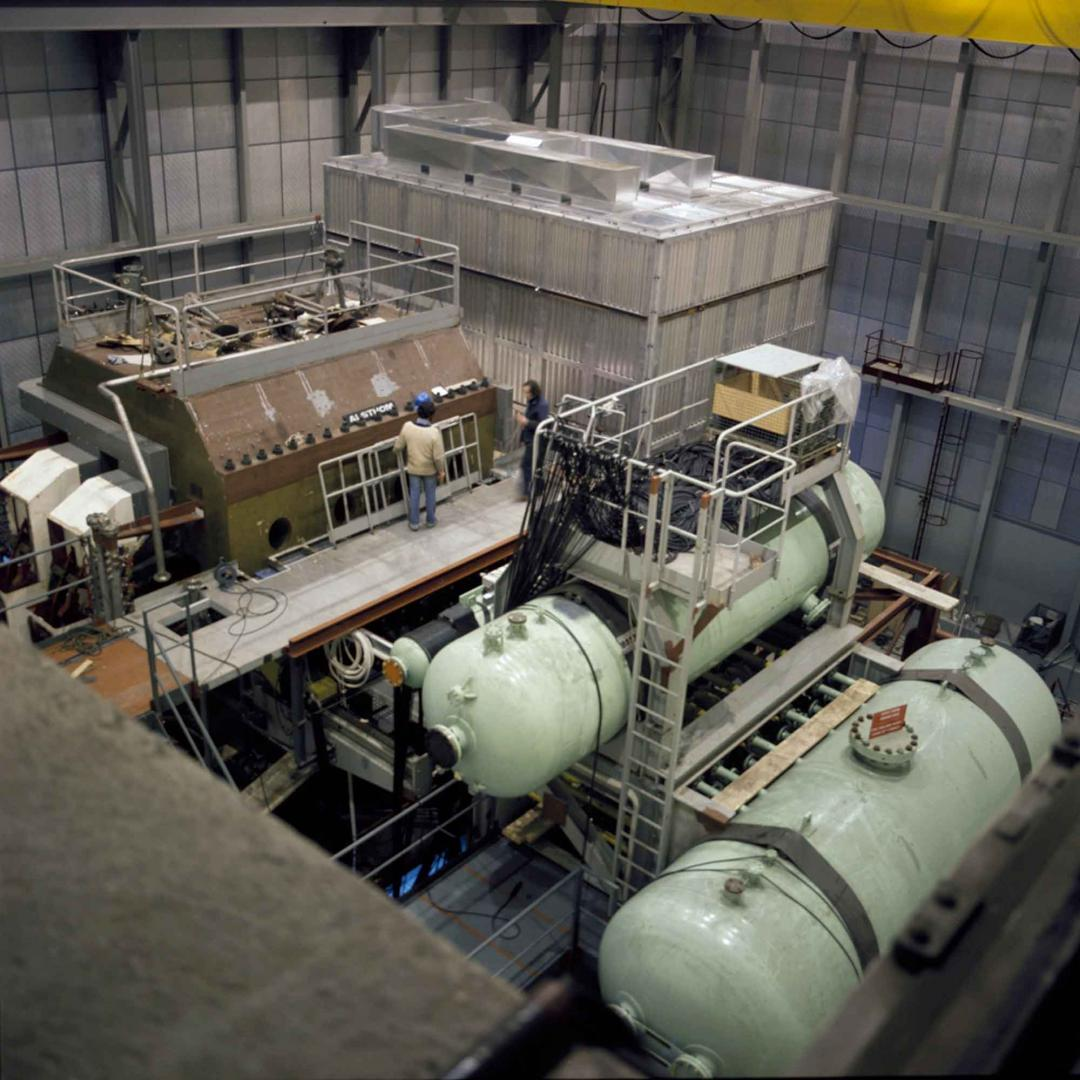
\includegraphics[width=\marginparwidth]{SM/gargamelle.jpg}
\captionof{figure}{Gargamelle.}
\label{GARGAMELLE}
}
\marginpar
{
\centering
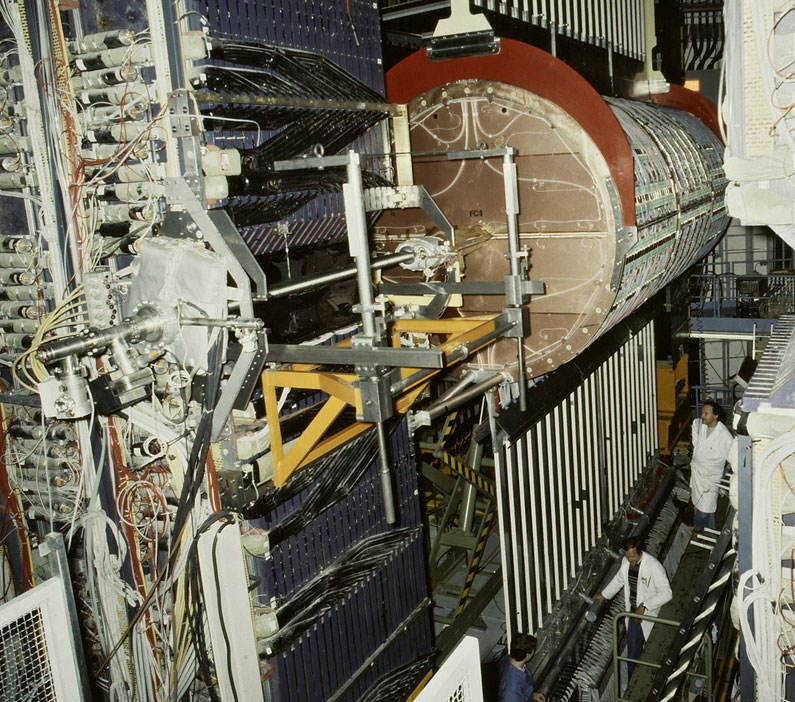
\includegraphics[width=\marginparwidth]{SM/ua1.jpg}
\captionof{figure}{UA1.}
\label{UA1}
}
\marginpar
{
\centering
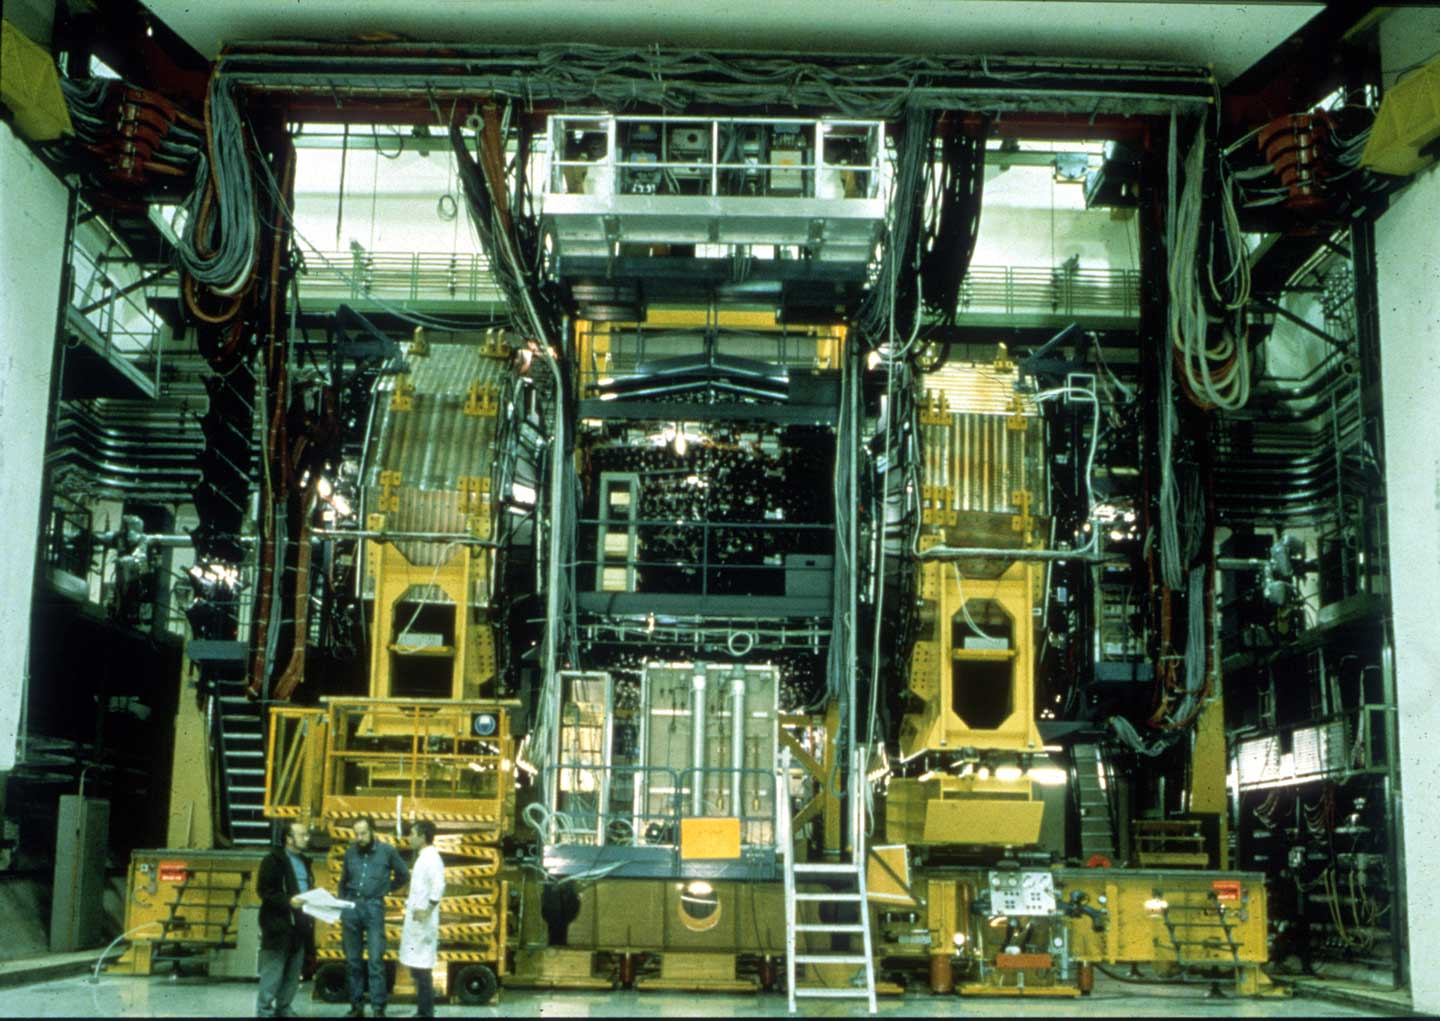
\includegraphics[width=\marginparwidth]{SM/ua2.jpg}
\captionof{figure}{UA2.}
\label{UA2}
}
\marginpar
{
\centering
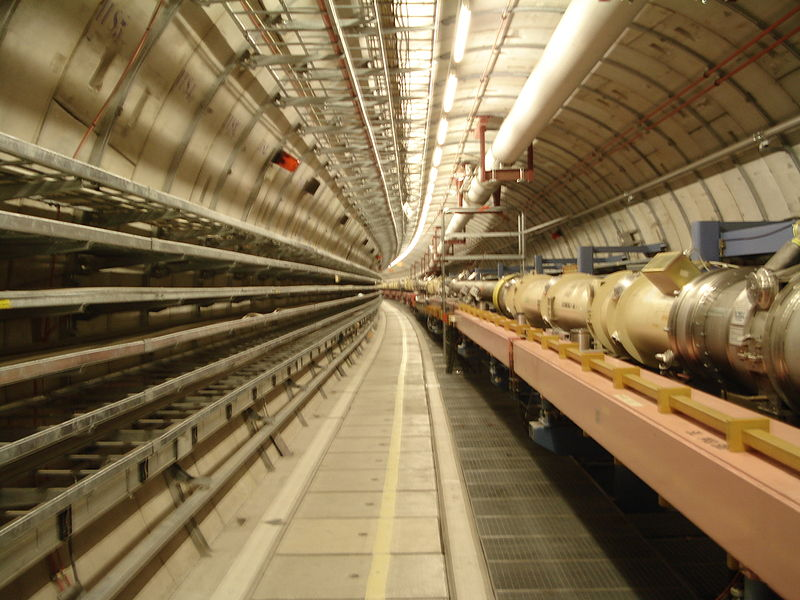
\includegraphics[width=\marginparwidth]{SM/HERA.jpg}
\captionof{figure}{tunnel du collisionneur HERA.}
\label{HERA}
}
\marginpar
{
\centering
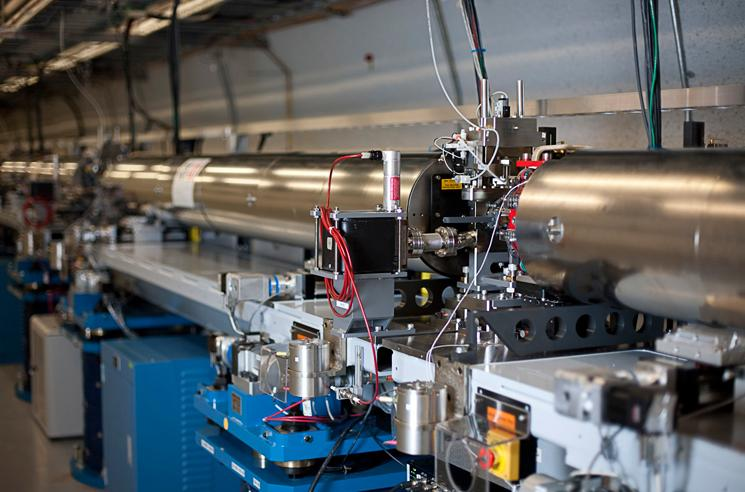
\includegraphics[width=\marginparwidth]{SM/slac.jpg}
\captionof{figure}{Beam line du SLAC.}
\label{SLAC}
} Dés 1932 Fermi essaya d'expliquer la désintégration nucléaire $\beta$ et l'interaction electromagnetique par des interactions à 4 points. Cette théorie  s'avérera être une théorie effective qui présente des divergences à haute énergie. Ce n'est que vers la fin des années 1960 que Glashow,Salam and Weinberg crée une théorie convaincante qui prédit la présence d'un courant neutre afin d'annuler les divergence du modèle. En 1973 't Hooft montra que cette théorie est libre renormalisable et parfaitement cohérente d'un point de vue théorique. La découverte expérimentale du courant neutre faible sera faite en 1973 au CERN par la chambre à bulle Gargamelle\ref{GARGAMELLE} conçue pour détecter les neutrinos. En 1983 les trois bosons du secteur électrofaible sont découverts au CERN grâce au expérience UA1\ref{UA1} et UA2\ref{UA2}.
De nombreuses mesures ont ensuite été effectuées par plusieurs collisionneurs: Large Electron Positron (LEP), Stanford Linear Collider (SLAC)\ref{SLAC}, Tevatron, Hadron-Elektron-Ringanlage (HERA)\ref{HERA}. Les propriétés des bosons $W^{\pm}$ et $Z^{0}$ ont été trouvées conformes au prédictions du Modèle Standard. 

De plus l'ensemble des mesures effectuées jusqu'à présent sont compatibles avec le Modèle Standard: La figure (fig.\ref{mesures}) montre la mesure de certains paramètres ainsi que leur "pull" défini par :
\begin{equation}
\frac{O^{mesure}-O^{fit}}{\sigma^{mesure}}
\end{equation}
c'est à dire la déviation entre les mesures expérimentales et les prédictions théoriques en unités de l'incertitude expérimentale. Tous les pulls sont inférieur à $3\sigma$. L'expérience et la théorie sont donc en très bon accord.
\begin{figure}[h!]
\centering
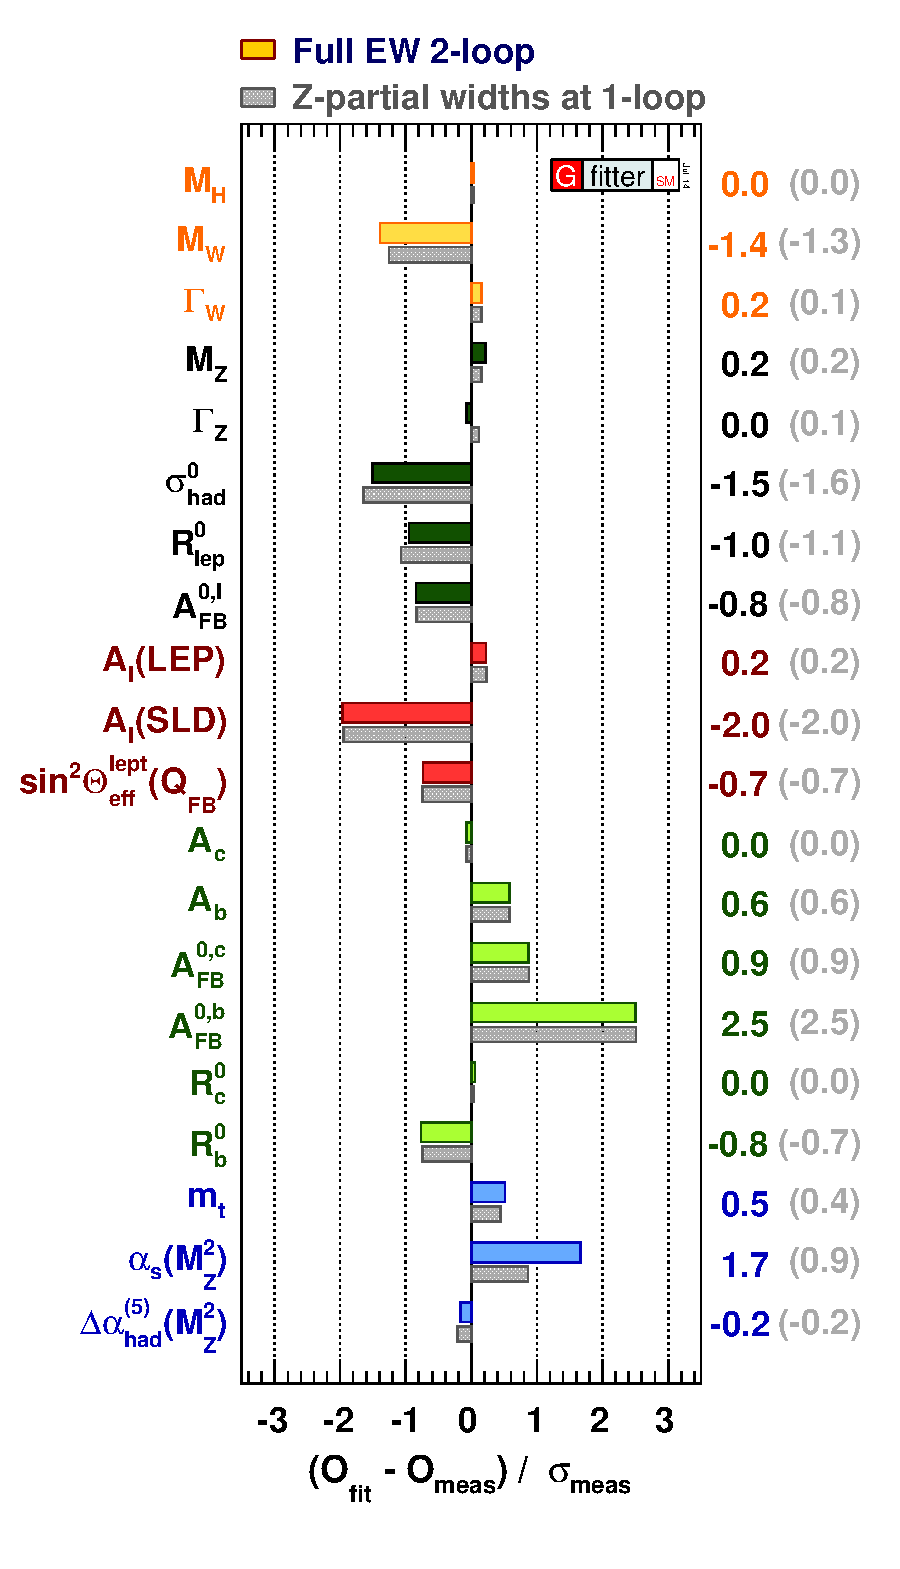
\includegraphics[width=0.45\textwidth]{SM/mesure.eps}
\captionof{figure}{Comparaison des résultats d'ajustement avec les mesures directes de certains paramètres du Modèle Standard.}
\label{mesures}
\end{figure}
\section{Les faiblesses du Modèle Standard}
Le modèle Standard est en accord remarquable avec l'expérience. Cependant, plusieurs problèmes et questions non résolubles amène à considérer le Modèle Standard comme une théorie effective, valable jusqu'à l'échelle du TeV. Une nouvelle physique qui engloberait le Modèle Standard devrait apparaitre à cette échelle d'énergie.

Parmis les principaux problèmes ou faits inexpliqués par le Modèle Standard, on peut citer :
\begin{itemize}[label=$\bullet$]
\item Les neutrinos massifs :\marginpar
{
\centering
\includegraphics[width=\marginparwidth]{SM/kamiokande.jpg}
\captionof{figure}{Intérieur du détecteur Super-Kamiokande.}
\label{kamiokande}
}
\marginpar
{
\centering
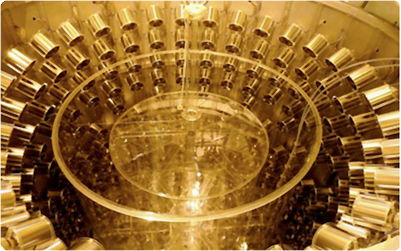
\includegraphics[width=\marginparwidth]{SM/chooz.jpg}
\captionof{figure}{Coeur du détecteur Double Chooz.}
\label{chooz}
} Les expérience Super-Kamiokande\ref{kamiokande} et GALLEX portant sur l'observation du flux de neutrinos provenant du Soleil et les expériences Double Chooz\ref{chooz} et K2K pour les flux de neutrinos de sources artificielles terrestres ont mis en évidence l'oscillation des neutrinos entre les saveurs leptoniques. Ces oscillations ne peuvent s'expliquer que si les neutrinos sont massifs et s'il existe des neutrinos droits. Bien que le Modèle Standard considére les neutrinos comme des particules de masse nulle et que de parité gauche, il est facile d'y ajouter un neutrino droit dans chaque famille et les couplages au doublet Higgs correspondant afin de rendre compte de ces faits expérimentaux\footnote{C'est d'ailleurs cette extension du Modèle Standard qui est présenté dans ce chapitre.}. Cependant cela aggrave le problème de la hiérarchie des masses car les masses des particules élémentaires s'étalent sur 10 ordres de grandeur !

\item Le nombre de paramètres libres : Le modèle standard contient 18 paramètres libres : les 3 constantes de couplages, les deux paramètres $\lambda$ et $\mu^2$ du potentiel de Higgs, 9 couplages de Yukawa et les trois angles et une phase pour les quarks dans la matrice CKM ainsi que l'angle associé auwx. Et d'autres encore en ajoutant le fait que les neutrinos soit massif.

\item Le nombre de familles : Le nombre de famille a été expérimentalement obtenu en comparant la section efficace hadronique en fonction de l'énergie du centre de masse expérimentale au prédiction théorique différents nombres de familles de neutrinos de masse négligeable. Actuellement on considère que trois familles\ref{neutrinos}. Cependant le fait que les neutrinos soient massif permet l'existance de plus de trois familles si les neutrinos on une masse supérieur à $m_{Z^{0}}/2$.
\begin{figure}[h!]
\centering
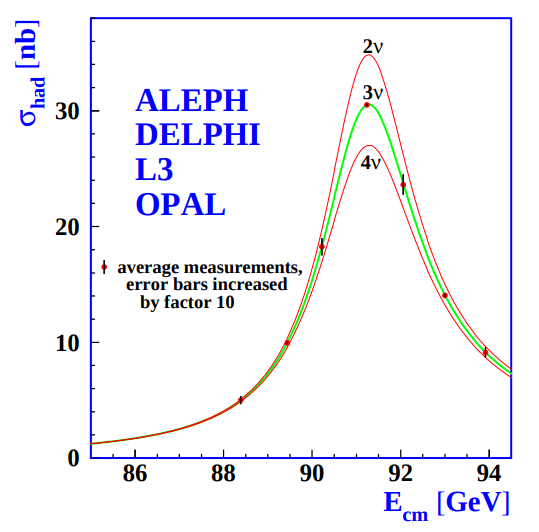
\includegraphics[width=0.30\textwidth]{SM/neutrinos.png}
\captionof{figure}{Mesures de la section efficace de production hadronique près de la résonance en Z. Les courbes indiquent les sections efficaces prédites pour deux,trois et quatres espéces de neutrinos avec les couplages du Modèle Standard et de masses négligeables.}
\label{neutrinos}
\end{figure}

\item La baryogénèse : Le Modèle Standard est incapable d'expliquer l'asymétrie entre la quantité de baryons (matière) et d'anti-baryons (anti-matière) observés dans l'Univers.

\item La gravitation : Le Modèle Standard ne comporte pas l'interaction gravitationnelle. Aucune formulation quantique de la gravitation n'a encore été trouvé. La meilleur théorie gravitationnelle, la relativité générale et malheureusement incompatible avec le Modèle Standard.

\item Le problème de naturalité : En effet, il paraît naturel de considérer une échelle d'énergie ou le Modèle Standard cesse d'être valide. Or, les ordres supérieur de la théorie perturbative ajoutent des corrections radiatives aux masses des différentes particules. En imposant une échelle d'énergie à la validité du Modèle Standard $\Lambda$, un "cut-off", les corrections vont en dépendre. Pour le boson de Higgs et en considérant les diagramme de la figure fig.\cref{corrections} on peut écrire :
\begin{equation}
m_{h}^{2}=m_{0}^{2}-\delta m_{h}^{2}
\end{equation}
avec $m_{0}^{2}$ la masse "nue" du boson, $m_{h}^{2}$ la masse effective et $\delta m_{h}^{2}$ les corrections radiative.
\begin{figure}[h!]
\centering
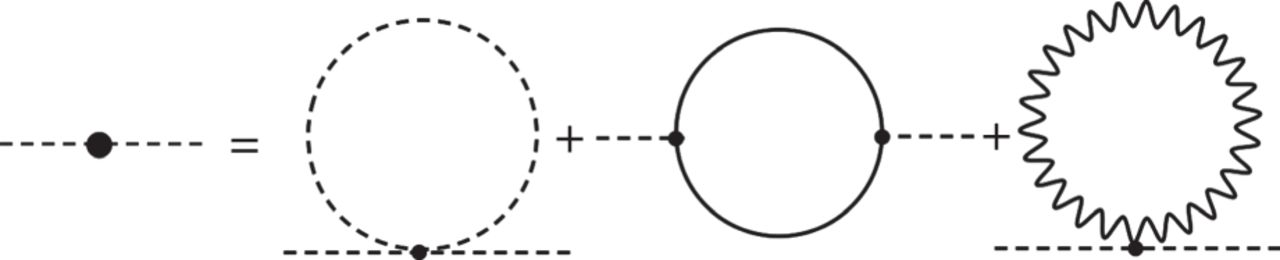
\includegraphics[width=1\textwidth]{SM/corrections.jpg}
\captionof{figure}{Correction radiative du premier ordre pour le boson de Higgs.}
\label{corrections}
\end{figure}
La contribution fermionique est de la forme :
\begin{equation}
\delta m_{h}^{2}=-\frac{y_{f}^{2}}{16\pi^{2}}\left(2\Lambda^{2}+\cdots\right)
\end{equation}
En considérant un cut-off de l'ordre de $\Lambda \sim 10^{16}$GeV il faut donc un accord à $10^{-30}$ entre $m_{0}^{2}$ et $\delta m_{h}^{2}$. Ce problème de hiérarchie, et de réglage fin des paramètres ne semble pas naturel.

\item Matière noire et Énergie noire : Des observations cosmologiques ont mis en évidence la présence de matière dite noire car elle n'émet pas et n'interagît pas avec les radiations électromagnétiques. Bien que n'ayant jamais été directement observé, son existence et certaines de ses propriétés peuvent être étudiés par leur effets gravitationnelles sur le mouvement de la matière visible, elle serait  également à l'origine de la formation des galaxies et des amas de galaxies, et de leurs répartition de façon non uniforme dans l'Univers. D'après les observations du satellite Plank\ref{Plank},
la matière que nous connaissons ne compose que 4.9\% du totale mass-énergie de l'Univers. La matière noire quant à elle ne compte que pour 26.8\%. Les 68.3\% restant sont composés d'énergie noire. Cette énergie serait responsable de l'accélération de  l'expansion de l'Univers qui à été mis en évidence en 1998 par les projets Supernova Cosmology Project et High-Z supernovae search team. Ni la matière noire ni l'énergie noire ne sont décrites par le Modèle Standard.
\marginpar
{
\centering
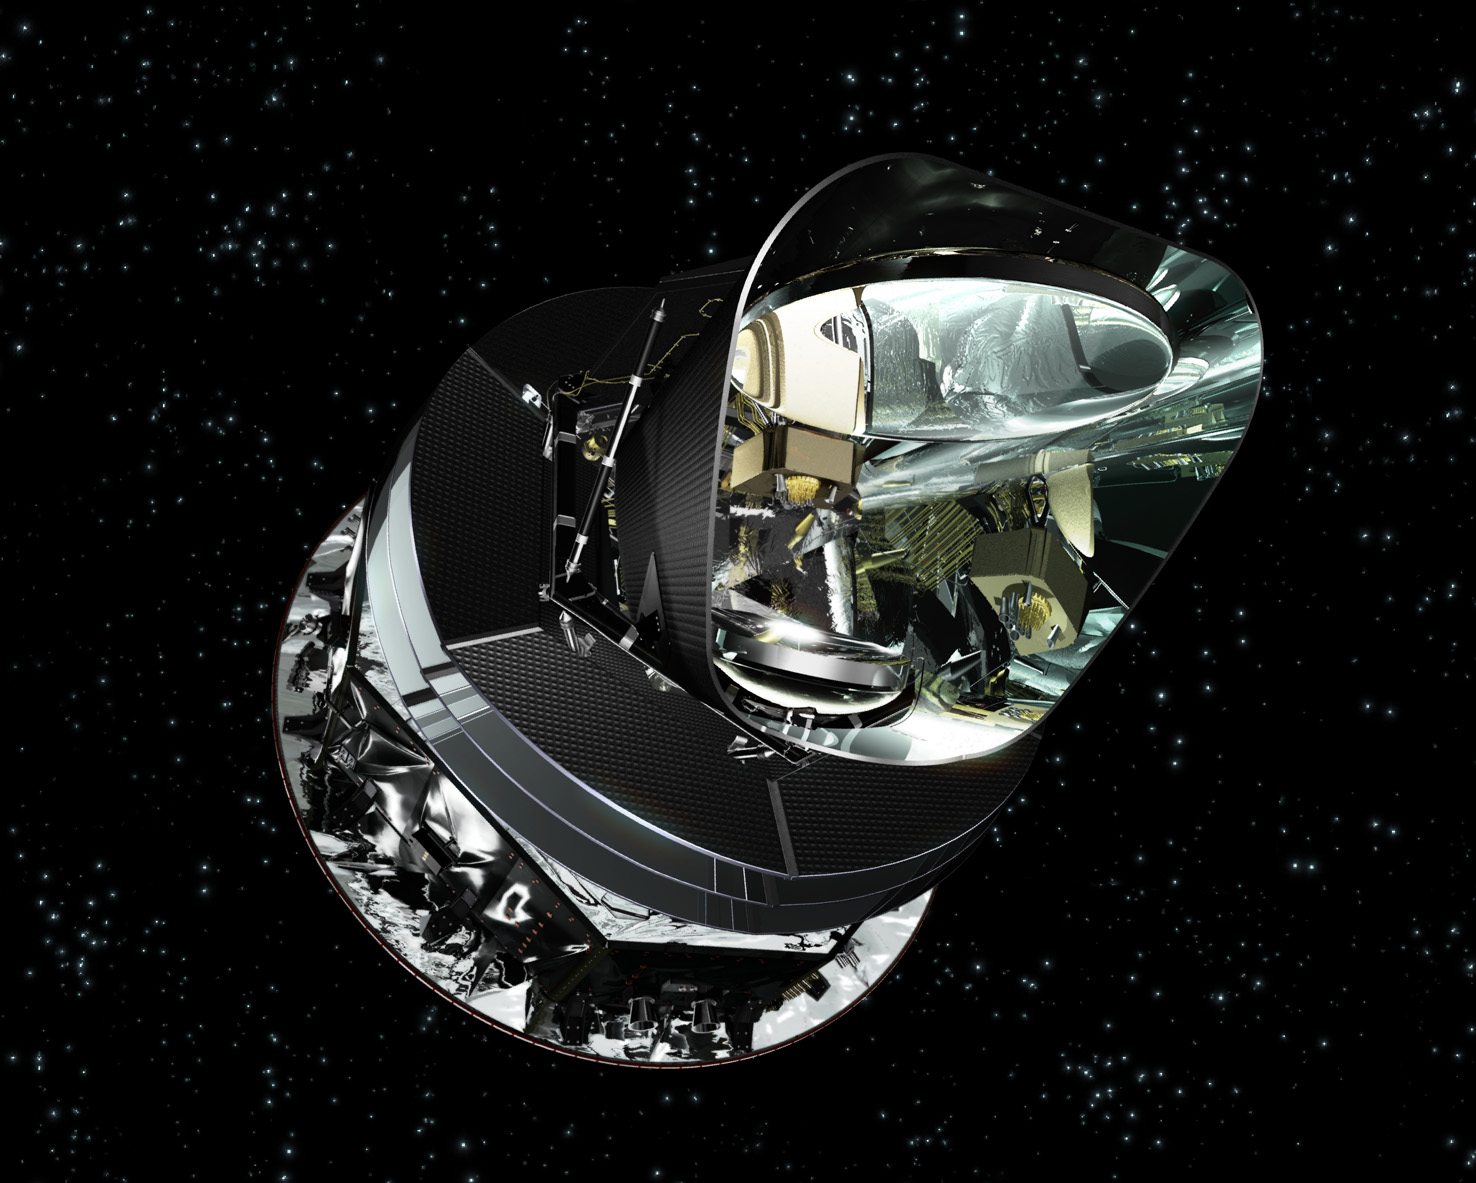
\includegraphics[width=\marginparwidth]{SM/plank.jpg}
\captionof{figure}{Le satellite Plank.}
\label{Plank}
} 
\end{itemize}